\section{Multiple correspondence analysis}\label{sec:mca}

Multiple \CA\ (MCA) is designed to display the relationships of the categories
of two or more discrete variables.  Again, there are several complementary
ways of defining MCA as an optimal scaling of categorical data.
The most typical starts by defining indicator (``dummy'') variables
for each category and reexpresses the \nway\ \ctab\ in the form
of a cases by variables indicator matrix, $\mat{Z}$.
Simple \CA\ for a two-way table can, in fact, be derived as the
canonical correlation analysis of the indicator matrix.
Unfortunately, the generalization to more than two variables follows
a somewhat different path, so that simple CA does not turn out to be
precisely a special case of MCA in some respects, particularly in the
decomposition of an interpretable \chisq\ over the dimensions in
the visual representation.

Nevertheless, MCA does provide a useful graphic portrayal of the
\emph{bivariate} relations among any number of categorical variables,
and has close relations to the mosaic matrix (\secref{sec:mosmat}).
And, if its limitations are understood, it may be helpful in
understanding large, multivariate categorical \Dsets.

\subsection{Bivariate MCA}\label{sec:mca-bi}
\ixon{multiple correspondence analysis!bivariate}
For the hair color, eye color data, the indicator matrix $\mat{Z}$
has 592 rows and $4+4=8$ columns.  The columns refer to the eight
categories of hair color and eye color and the rows to the students
in Snee's \citeyear{Snee:74} sample.
The indicator matrix is shown in \tabref{tab:haireye2}, where
to save space each combination of hair color and eye color actually
corresponds to the number of repeated rows represented by the $n_{ij}$
column.
Variable $h_1$ represents the hair category Black, and
Variable $e_1$ represents the eye category Brown,
so the first row of table \tabref{tab:haireye2}
corresponds to the 68 people with black hair and brown eyes.
The indicator matrix $\mat{Z}$ thus has 68 identical rows with that response
pattern.
\begin{table}[htb]
 \caption{Indicator matrix for hair color, eye color data (grouped)}\label{tab:haireye2}
 \begin{center}
 \begin{tabular}{|ll r | rrrr|rrrr|}
 \hline
       &     &     & \multicolumn{4}{c|}{Hair} & \multicolumn{4}{c|}{Eye} \\
  Hair & Eye & $n_{ij}$ 
  & $h_1$ & $h_2$ & $h_3$ & $h_4$ 
  & $e_1$ & $e_2$ & $e_3$ & $e_4$ 
  \\ 
 \hline
  BLACK & Brown &  68 & 1 & 0 & 0 & 0 & 1 & 0 & 0 & 0 \\ 
  BROWN & Brown & 119 & 0 & 1 & 0 & 0 & 1 & 0 & 0 & 0 \\ 
  RED   & Brown &  26 & 0 & 0 & 1 & 0 & 1 & 0 & 0 & 0 \\ 
  BLOND & Brown &   7 & 0 & 0 & 0 & 1 & 1 & 0 & 0 & 0 \\  [1mm]
  BLACK & Hazel &  15 & 1 & 0 & 0 & 0 & 0 & 1 & 0 & 0 \\ 
  BROWN & Hazel &  54 & 0 & 1 & 0 & 0 & 0 & 1 & 0 & 0 \\ 
  RED   & Hazel &  14 & 0 & 0 & 1 & 0 & 0 & 1 & 0 & 0 \\ 
  BLOND & Hazel &  10 & 0 & 0 & 0 & 1 & 0 & 1 & 0 & 0 \\  [1mm]
  BLACK & Green &   5 & 1 & 0 & 0 & 0 & 0 & 0 & 1 & 0 \\ 
  BROWN & Green &  29 & 0 & 1 & 0 & 0 & 0 & 0 & 1 & 0 \\ 
  RED   & Green &  14 & 0 & 0 & 1 & 0 & 0 & 0 & 1 & 0 \\ 
  BLOND & Green &  16 & 0 & 0 & 0 & 1 & 0 & 0 & 1 & 0 \\  [1mm]
  BLACK & Blue  &  20 & 1 & 0 & 0 & 0 & 0 & 0 & 0 & 1 \\ 
  BROWN & Blue  &  84 & 0 & 1 & 0 & 0 & 0 & 0 & 0 & 1 \\ 
  RED   & Blue  &  17 & 0 & 0 & 1 & 0 & 0 & 0 & 0 & 1 \\ 
  BLOND & Blue  &  94 & 0 & 0 & 0 & 1 & 0 & 0 & 0 & 1 \\ 
 \hline
 (Totals) &       & 592 
 & 220 & 215 & 93 & 64 
 & 108 & 286 & 71 & 127 
 \\ 
 \hline
 \end{tabular}
 \end{center}
\end{table}




Each row of the indicator matrix sums to 2, the number of variables
represented, and each category column sums to the marginal total for
that category.
Note that appropriate subsets of the rows are in a sense synonymous with
the column categories.  For example, the first four rows of the table
are all those with brown eyes, so these rows represent $e_1$.

If the indicator matrix is partitioned as
$\mat{Z} = [ \mat{Z}_1 , \mat{Z}_2 ]$, corresponding to the two sets of
categories, then the contingency table is given by
$\mat{N} = \mat{Z}_1 \trans \mat{Z}_2$.
Then, MCA can be described as the application of the simple \CA\
algorithm to the indicator matrix $\mat{Z}$.
This analysis would yield scores for the rows of $\mat{Z}$ (the cases)
and for the columns (the categories).
As in simple CA, each row point is the weighted average of the scores
for the column categories, and each column point is the weighted average
of the scores for the row observations.

Consequently, the point for any category is the centroid of all the
observations with a response in that category, and
all observations with the same response pattern coincide.
As well, the origin reflects the weighted average of the categories for
\emph{each} variable.  As a result, category points with low marginal
frequencies will be located further away from the origin,
while categories with high marginal frequencies will be closer to the
origin.
For a binary variable, the two category points will appear on a line
through the origin, with distances inversely proportional to their
marginal frequencies.

\begin{Example}[haireye4]{Hair color and eye color}
For expository purposes,
we illustrate the analysis of the indicator matrix below for the hair color,
eye color data.
MCA is usually carried out more simply through analysis of
the ``Burt matrix'', described in the following subsection.

The indicator matrix may be constructed from the \Dset\ in \ctab\ form
as shown below, using \PROC{TRANSPOSE} and a \Dstp\ to calculate
the dummy variables from the original row and column variables.%
\footnote{These steps actually create a design matrix, with one
observation per category, with the frequencies, $n_{ij}$, as shown in
\tabref{tab:haireye2}.  In the \pname{\%corresp} step, the
\pname{count} variable is used as a weight, to reproduce the
indicator matrix.}
%% input: /Users/friendly/sasuser/catdata/mcahair.sas
%% last modified: 24-Jul-99 11:19
\begin{listing}
data haireye;
   input  EYE $ BLACK BROWN RED BLOND ;
datalines;
         Brown    68   119    26     7    
         Hazel    15    54    14    10    
         Green     5    29    14    16    
         Blue     20    84    17    94    
;
*-- Reshape data to frequency form;
proc transpose data=haireye out=haireye2;
   var BLACK BROWN RED BLOND;
   by eye notsorted;

*-- Create dummy variables;
data haireye2;
   set haireye2 (rename= (_name_=hair col1=count));
   h1 = (hair='BLACK');   h2 = (hair='BROWN');
   h3 = (hair='RED');     h4 = (hair='BLOND');
   e1 = (eye ='Brown');   e2 = (eye ='Hazel');
   e3 = (eye ='Green');   e4 = (eye ='Blue');
\end{listing}


Analysis of the indicator matrix (the \Dset\ \pname{haireye2})
is conveniently carried out with the \macro{CORRESP}.
\begin{listing}
axis1 length=6.5 IN order=(-1.2 to 2 by 0.4) label=(a=90);
axis2 length=6.5 IN order=(-1.2 to 2 by 0.4);

%corresp(data=haireye2, id=id, var=h1-h4 e1-e4, weight=count,
   symbols=none dot, pos=5 -, vaxis=axis1, haxis=axis2, anno=labels, gplot=no);
\end{listing}

Some additional Annotation steps (not shown) to add some lines to
the \ADS\ \pname{labels} produces \figref{fig:mcahair},
in which the row and column points are shown in principal coordinates.
Comparing this with \figref{fig:corresp3}, we see that the pattern of
the hair color and eye color categories is the same in the analysis of
the contingency table (\figref{fig:corresp3}) and the analysis of the
indicator matrix (\figref{fig:mcahair}), except that the axes are scaled
differently---the display has been stretched along the second (vertical)
dimension.
Indeed, it may be shown \citep{Greenacre:84}
that the two displays are identical, except for changes in scales along
the axes.
There is no difference at all between the displays in standard coordinates.
\citet[pp. 130--134]{Greenacre:84} describes the precise relations
between the geometries of the two analyses.

%% one figure
\begin{figure}[htb]
  \centering
  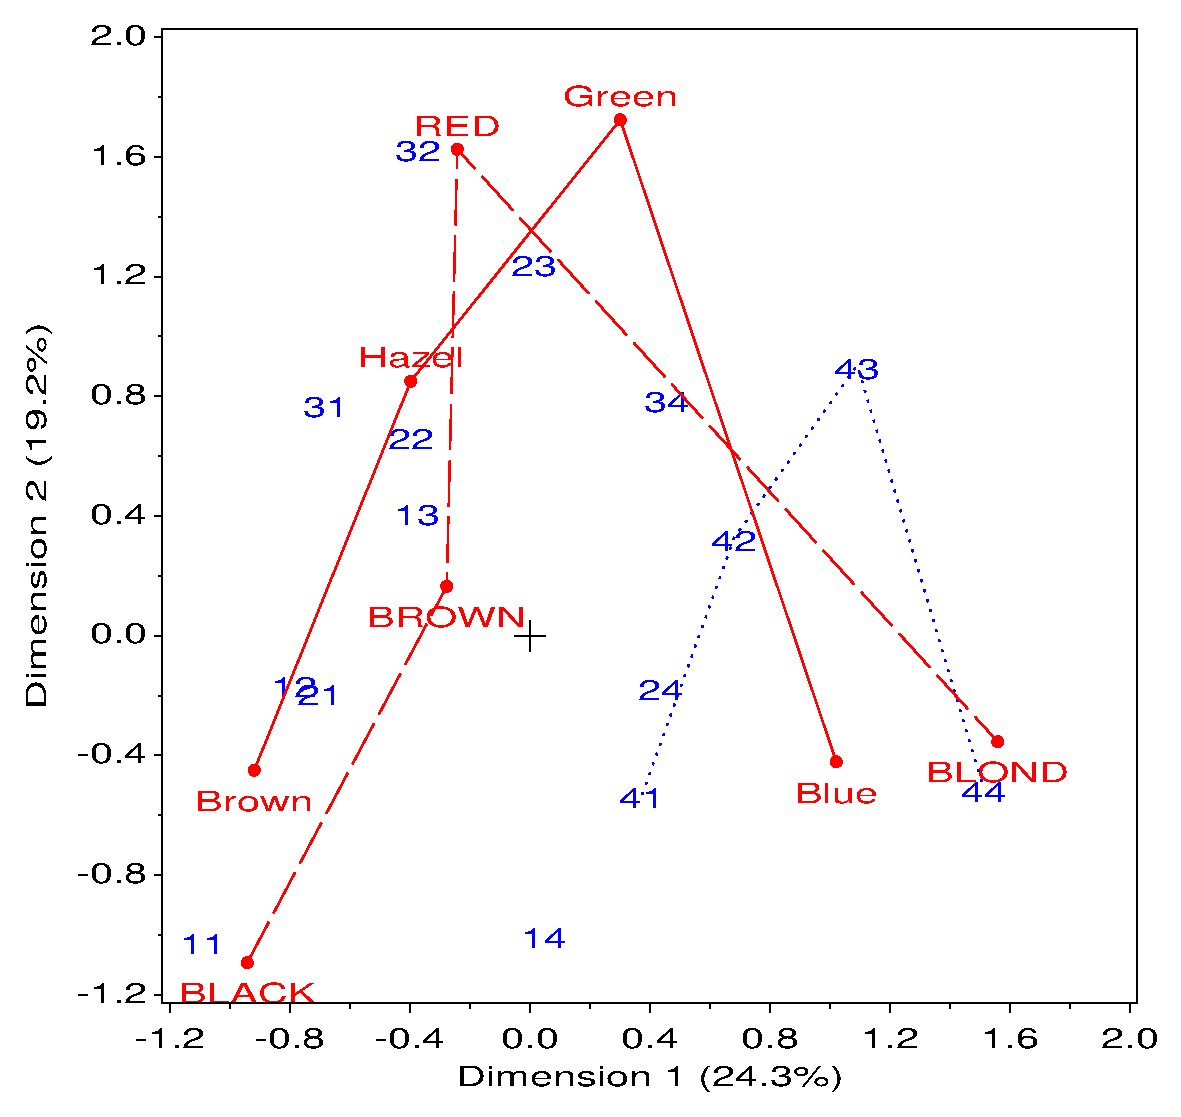
\includegraphics[scale=.7,clip]{ch5/fig/mcahair}
  \caption[Correspondence
  analysis of the indicator matrix Z for the hair color, eye color data]{Correspondence
  analysis of the indicator matrix $\mat{Z}$ for the hair color, eye color data.
  The category points are joined for the hair color and eye color categories.
  Observation (row) points, are labeled by the subscripts of $h, e$.
  The dotted line connects those with blond hair.}%
  \label{fig:mcahair}
\end{figure}

\figref{fig:mcahair} also plots the row points (corresponding to the observations) from this analysis.  Each point is labeled by the subscripts,
$ij$, of $h_i e_j$, and actually represents $n_{ij}$ rows
from the indicator matrix
plotted at the point.  For example, the points labeled `41'--`44'
represent all the observations with blond hair.
There are actually 94 observations at the point `44', representing the
blue-eyed blonds.
\end{Example}


A major difference between analysis of the \ctab\ and analysis of the
indicator matrix is in the decomposition of inertia and $\chisq$
for the dimensions.
The inertias for the analysis of the indicator matrix are shown in
\outref{out:mcahair.1}.
Comparing these values with \outref{out:corresp3.1},
we see that 6 dimensions are shown in the analysis of the indicator matrix,
while only 3 are shown in the analysis of the \ctab.
The inertias and $\chisq$ values differ less dramatically than
in \outref{out:corresp3.1}, and the inertias sum to exactly 3.0 in the
indicator matrix analysis.

For a two-way table of size ($J_1 \times J_2$), CA of the indicator matrix
produces $J_1 + J_2 - 2$ dimensions, but it turns out that half of these
are artifacts which should be disregarded, and these correspond to those
with principal inertias $\lambda^2 < \frac{1}{2}$.
The total inertia depends not on the $\chisq$ for association
as in simple CA of the \ctab,
but is simply $(J_1 + J_2 - 2) / 2$.
The singular values of the non-trivial dimensions in the
analysis of $\mat{Z}$ (symbolized as $\lambda_i^Z$)
are related to those ($\lambda_i$) of the analysis of the \ctab\ by
\begin{equation*}%\label{eq:lzn}
 \lambda_i^Z = \{ \frac{1}{2} [ 1 + \lambda_i ] \}^{1/2}
 \period
\end{equation*}
We can recover the singular values from the analysis of the \ctab\
by inverting this relation, which gives
\begin{equation}\label{eq:lnz}
 \lambda_i = 2  (\lambda_i^Z)^2 - 1
 \period
\end{equation}
For example, using the first singular value, $\lambda_1^Z = 0.8535$ from
\outref{out:mcahair.1} in \eqref{eq:lnz}
gives $\lambda_1 = 2 ({0.8535} ^ 2) - 1 =  0.4569$,
the value in \outref{out:corresp3.1}.

\begin{Output}[htb]
\caption{Correspondence analysis output for the indicator matrix of the hair color, eye color data}\label{out:mcahair.1}
\small
\verbatiminput{ch5/out/mcahair.1}
\end{Output}

%\begin{Output}[htb]
%\caption{Correspondence analysis output, row and column scores, for the hair color, eye color data}\label{out:mcahair.2}
%\small
%\verbatiminput{ch5/out/mcahair.2}
%\end{Output}

\subsection{The Burt matrix}\label{sec:mca-burt}
\ixon{Burt matrix}
The same solution for the category points as in the
analysis of the indicator matrix may be obtained more simply
from the so-called ``Burt matrix'' \citep{Burt:50},
\begin{equation*}%\label{eq:burt2}
 \mat{B} = \mat{Z}\trans \mat{Z}
 =
 \left[
 \begin{array}{ll}
 \mat{N}_{1} & \mat{N} \\
 \mat{N}\trans & \mat{N}_{2} \\
 \end{array}
 \right]
 \comma
\end{equation*}
where $\mat{N}_{1}$ and $\mat{N}_{2}$ are diagonal matrices containing
the marginal frequencies of the two variables (the column sums of
$\mat{Z}_1$ and $\mat{Z}_2$).

The standard coordinates from an analysis of the Burt matrix
$\mat{B}$ are identical to those of $\mat{Z}$.
The singular values of $\mat{B}$ are the squares of those of $\mat{Z}$;
however, the \proc{CORRESP} compensates by taking the square root,
so the same values are printed.

The \proc{CORRESP} and the \macro{CORRESP} calculate the
Burt matrix when the \opt{MCA}{CORRESP} is used, and the category
variables are given in the \stmt{TABLES}{CORRESP}.
For the hair color, eye color data, we obtain the same category points
and inertias as the analysis in \exref{ex:haireye4} with the following
statement, using the table variables \pname{hair} and \pname{eye},
rather than the indicator variables \pname{H1-H4 E1-E4}.
\begin{listing}
%corresp(data=haireye2, tables=hair eye, weight=count, options=short mca,
   inc=0.4, xextra=0 1, pos=-, symbols=dot, colors=red);
\end{listing}
The Burt matrix is symmetric and the rows and columns both refer to
the hair, eye categories.
Only the column (category) points appear in the output and the plot.
\ixoff{multiple correspondence analysis!bivariate}

\subsection{Multivariate MCA}\label{sec:mca-multi}
The coding of categorical variables in an indicator matrix provides
a direct and natural way to extend this analysis to more than two variables.
If there are $Q$ categorical variables, and variable $q$ has $J_q$
categories, then the $Q$-way \ctab, of size
$J = \prod_{q=1}^Q J_q = J_1 \times J_2 \times \cdots \times J_Q$,
with a total of $n = n_{++\cdots}$ observations
may be represented by the partitioned $(n \times J)$ indicator matrix
$[ \mat{Z}_1 \, \mat{Z}_2  \, \dots \, \mat{Z}_Q ]$.

Then the Burt matrix is the symmetric partitioned matrix
\begin{equation*}
 \mat{B} = \mat{Z}\trans \mat{Z}
 =
 \left[
 \begin{array}{llll}
 \mat{N}_{[1]} & \mat{N}_{[12]} & \cdots & \mat{N}_{[1Q]}\\
 \mat{N}_{[21]} & \mat{N}_{[2]} & \cdots & \mat{N}_{[2Q]}\\
 \vdots        & \vdots         & \ddots  & \vdots       \\
 \mat{N}_{[Q1]} & \mat{N}_{[Q2]} & \cdots & \mat{N}_{[Q]}\\
 \end{array}
 \right]
 \comma
\end{equation*}
where again the diagonal blocks $\mat{N}_{[i]}$ contain the one-way
marginal frequencies.

Classical MCA (see, e.g., \cite{Greenacre:84,GowerHand:96})
can then be defined as a singular value decomposition of the matrix $\mat{B}$ which produces scores for the
categories of all variables so that the greatest proportion of the
bivariate, pairwise associations in all off-diagonal blocks is accounted for in
a small number of dimensions.
In this respect, MCA resembles multivariate methods for quantitative
data based on the joint bivariate correlation or covariance matrix
($\mat{\Sigma}$)
and there is some justification to regard the Burt matrix as the
categorical analog of $\mat{\Sigma}$.%
\footnote{For multivariate normal data, however, the mean vector and
covariance matrix are sufficient statistics, so all higher-way relations
are captured in the covariance matrix.  This is not true of the Burt
matrix.}

There is a close connection between this analysis and the bivariate mosaic
matrix (\secref{sec:mosmat}):
The mosaic matrix displays the residuals from independence for each
pair of variables, and thus provides a visual representation of the Burt matrix.
(The representation would be complete if the one-way margins
were drawn in the diagonal cells.)
The total amount of shading in all the individual mosaics
portrays the total pairwise associations decomposed by MCA.
See \citet{Friendly:99b} for further details.

In \secref{sec:mca-bi} we saw that, with $Q=2$ categorical variables,
analysis of the indicator matrix or the Burt matrix
produces twice as many dimensions as the analysis of the
equivalent \ctab; but only those whose principal inertias,
$(\lambda^Z)^2$, exceed $\frac{1}{2}$
are interesting, the remaining ones being artifacts.
When there are $Q>2$ variables represented in the Burt matrix,
it may be argued \citep{Greenacre:84,Greenacre:90} that the
interesting dimensions correspond to those with principal
inertia $> 1/Q$.

A more serious problem lies in the calculation of total inertia,
and therefore in the chi-square values and corresponding percentages
of association accounted for in some number of dimensions.
In simple CA, the total inertia is $\chisq /n$, and it therefore
makes sense to talk of percentage of association accounted for
by each dimension.
But in MCA of
the Burt matrix (with the square-root fixup provided by the \proc{CORRESP}),
the total inertia is simply $(J - Q)/Q = J/Q - 1$,
because that is what the analysis of the equivalent indicator matrix
would give.
The consequence is that the $\chisq$ percentages reported by
\PROC{CORRESP} are somewhat misleading, and give a rather pessimistic
view of the association accounted for in the two (or three) dimensions
usually plotted.
\ixoff{Burt matrix}

To more adequately reflect the percentage of association in MCA,
\citet{Benzecri:77} suggested the calculation of
\begin{equation*}%\label{eq:benzecri}
(\lambda_i^{\star})^2 =
{\left[ \frac{Q}{Q-1} ( \lambda_i^Z - (1/Q) ) \right]}^2
\end{equation*}
as the principal inertia due to the dimensions with $(\lambda^Z)^2 > 1/2$.
Benz{\'e}cri then expresses the contribution of each dimension as
$ (\lambda_i^{\star})^2 / \sum (\lambda_i^{\star})^2$,
with the summation over only dimensions with $(\lambda^Z)^2 > 1/2$.

Although this \emph{is} an improvement, it is somewhat \emph{ad hoc},
and not totally satisfactory.
\citet{Greenacre:88} develops an alternative analysis
called joint correspondence analysis (JCA)
which fits only the $Q \times (Q-1) /2$ off-diagonal blocks
of the Burt matrix.
\ix{correspondence analysis!joint}
\citet{Greenacre:90} then proposed to define the total inertia
as the average inertia in these off-diagonal blocks.%
\footnote{In \sasver{8}, the \proc{CORRESP} provides the
\pname{BENZECRI} and \pname{GREENACRE} options, which give more
reasonable and useful inertia contributions.
\ix{CORRESP@\texttt{CORRESP} procedure!GREENACRE@\texttt{GREENACRE} option}
\ix{CORRESP@\texttt{CORRESP} procedure!BENZECRI@\texttt{BENZECRI} option}
One of these options should be used for MCA in the \mparm{OPTIONS}{CORRESP}
with the \macro{CORRESP}.
}

For the interpretation of MCA plots, we note the following relations
\citep[\S 5.2]{Greenacre:84}:
\begin{itemize*}
\item The centroid of the categories for each discrete variable
is at the origin of the display.
\item The inertia contributed by a given variable increases with the
number of response categories.
\item For a particular variable,
the inertia contributed by a given category increases as the marginal
frequency in that category \emph{decreases}.
\item The category points for a binary variable lie on a line
through the origin.  The distance of each point to the origin is
inversely related to the marginal frequency.
\end{itemize*}

\begin{Example}[titanic2]{Survival on the \emph{Titanic}}
An MCA analysis of the \emph{Titanic} data is carried out
using the \opt{MCA}{CORRESP} of \PROC{CORRESP} as follows:

\begin{listing}
%include catdata(titanic);
proc corresp data=titanic short mca outc=coords;
   weight count;
   tables age sex class survive;
   run;
\end{listing}
\begin{Output}[htb]
\caption{Chi-Square Decomposition for \emph{Titanic} MCA}\label{out:titanicmca1}
\begin{output}
                      Inertia and Chi-Square Decomposition

        Singular  Principal Chi-
        Values    Inertias  Squares Percents    6   12   18   24   30
                                            ----+----+----+----+----+---
        0.66714   0.44508   4609.06  29.67% *************************
        0.55231   0.30504   3158.90  20.34% *****************
        0.50001   0.25001   2588.96  16.67% **************
        0.45281   0.20504   2123.28  13.67% ***********
        0.42251   0.17852   1848.63  11.90% **********
        0.34105   0.11632   1204.54   7.75% ******
                  -------   -------
                  1.50000   15533.4 (Degrees of Freedom = 81)
\end{output}
\end{Output}
The printed output, shown partially in \outref{out:titanicmca1}--\ref{out:titanicmca2}
suggests that two dimensions accounts for
50\% of the total association ($\chi^2 (81) = 15533.4$), representing
all pairwise interactions among the four factors.
As noted earlier, this assessment is highly pessimistic,
because of the artificial dimensions induced in the MCA solution
by the diagonal blocks of the Burt matrix.  The suggestion
\citep[p. 145]{Greenacre:84} that we only consider dimensions whose
principal inertias exceed $1/Q = 0.25$ suggests that two dimensions
are sufficient here.
\ix{Burt matrix}

\figref{fig:titanicmca} shows the 2-dimensional solution.
The points for each factor have the property that the sum of coordinates
on each dimension, weighted inversely by the marginal proportions, equals
zero, so that high frequency categories (e.g., Adult) are close to the origin.
The first dimension is perfectly aligned with the Gender factor, and also
strongly aligned with Survival.  The second dimension pertains mainly to
Class and Age effects.  Considering those points which differ from the
origin most similarly (in distance and direction) to the point for Survived,
gives the interpretation that survival was associated with being female
or upper class or (to a lesser degree) being a child.

\begin{figure}[htb]
  \centering
  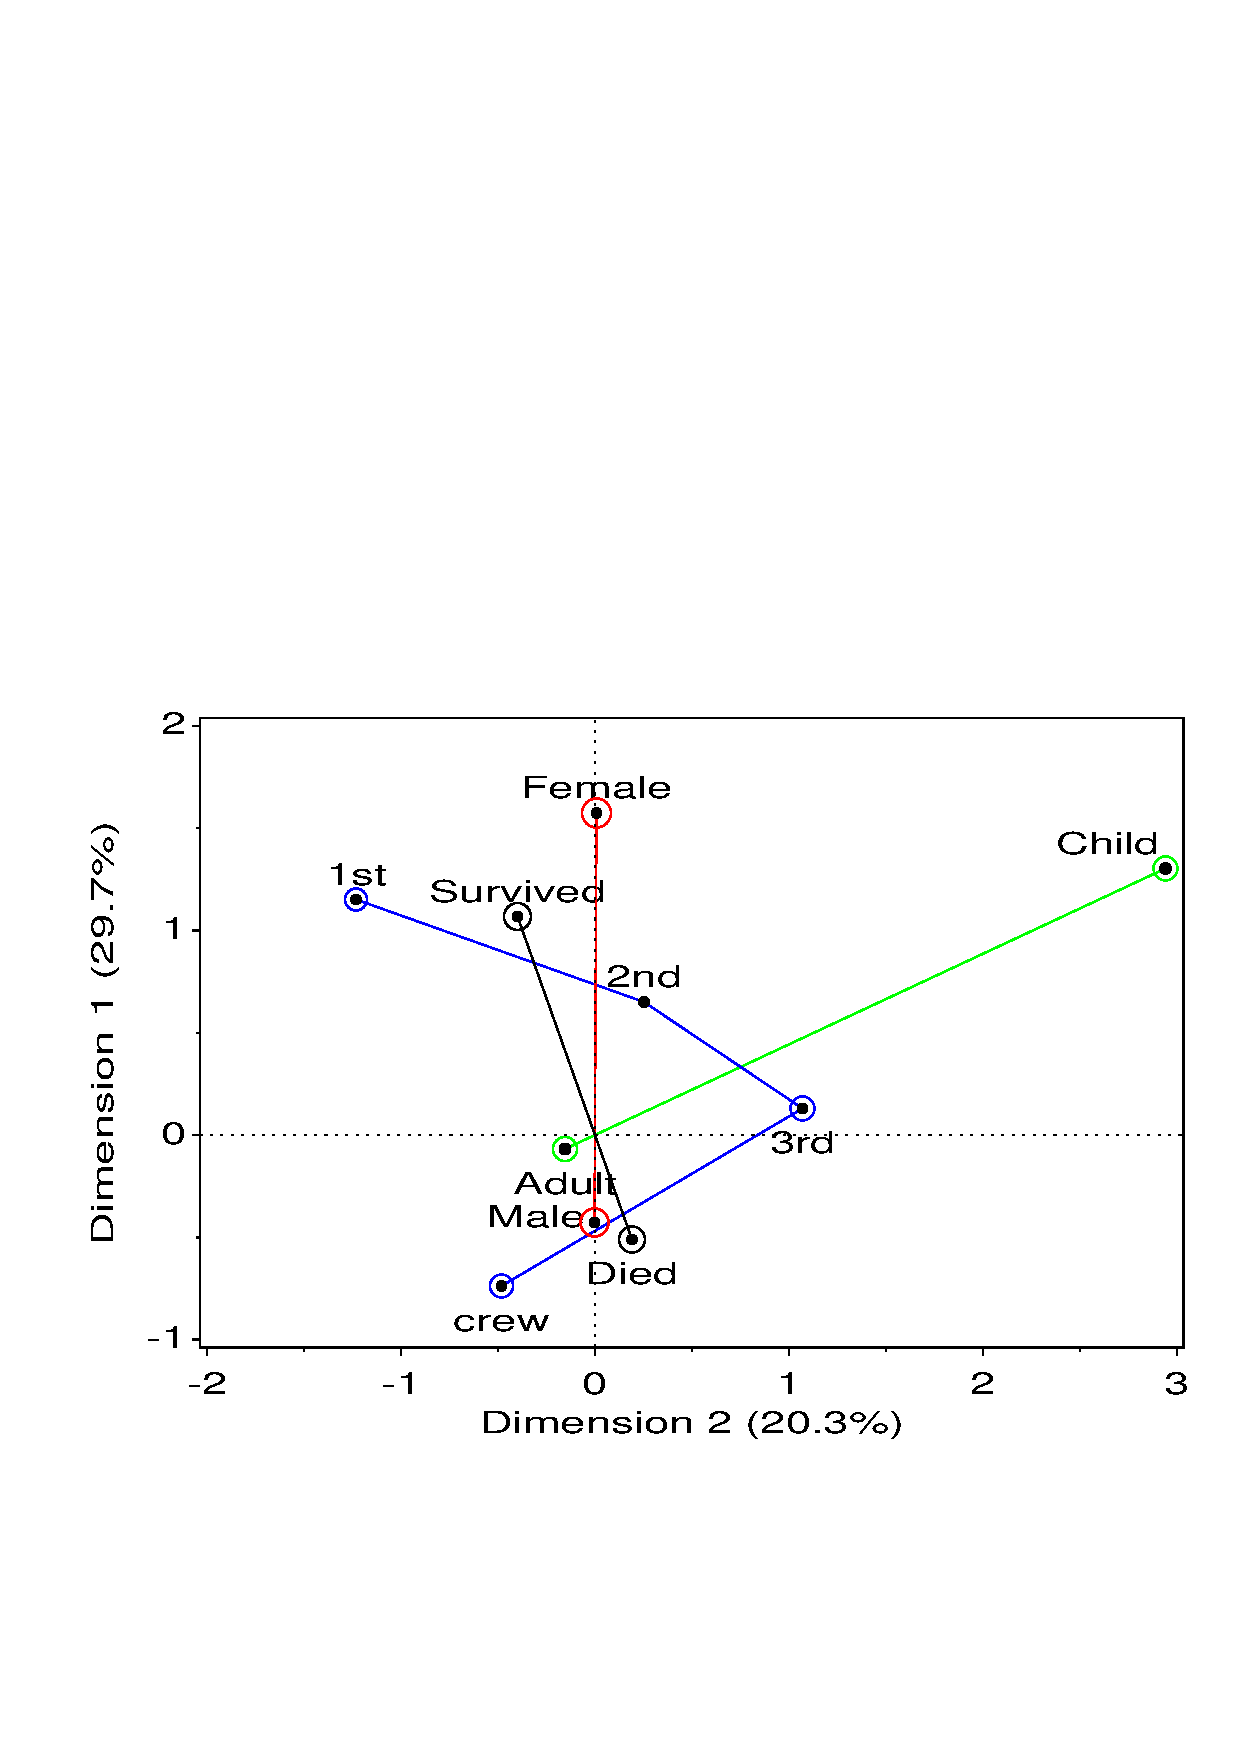
\includegraphics[scale=.8,clip]{ch5/fig/titanicmca}
  \caption{Titanic data: MCA analysis}\label{fig:titanicmca}
\end{figure}

%% input: /users/faculty/friendly/sasuser/catdata/titanicmca.sas
%% last modified: 04-Aug-98 17:16
\begin{listing}
data coords;
   set coords;
   where (_type_) = 'VAR';
   keep _name_ factor dim1-dim2 quality dist;
   dist = sqrt(dim1**2 + dim2**2);
   select;
      when (_name_ in ('Adult', 'Child'))   factor = 'Age    ';
      when (_name_ in ('Female', 'Male'))   factor = 'Sex    ';
      when (_name_ in ('Died', 'Survived')) factor = 'Survive';
      otherwise                             factor = 'Class';
      end;

proc sort;
   by factor;
proc print;
   id _name_;
%label(data=coords, x=dim2, y=dim1, text=_name_,
   pos=-, out=labels);

data labels;
   set labels;
   if text='Male' then do;
      x = x-.3;
      y = y+.2;
      end;

*-- join pairs of points representing the same variable;
data join;
   set coords;
   by factor;
   length function $8;
   xsys='2'; ysys='2';
   colors='green blue magenta red ';
   if first.factor then g+1;
   color = trim(scan(colors,g));
   x = dim2; y = dim1;
   if first.factor
      then function='move';
      else function='draw';
   output;
   *-- circle proportional to quality;
   size = .5 + 3*quality;
   text = 'circle';
   function = 'symbol';
   output;

data labels;           /* Concatenate the annotate data sets */
   set labels join;

title lspace=3.2in 'Survival on the Titanic';
proc gplot data=coords;
   plot dim1 * dim2 
      / frame href=0 vref=0 lvref=34 lhref=34
      vaxis=axis1 haxis=axis2 hm=1 vm=1
      anno=labels;
   symbol1 v=dot h=1;
   axis1 length=4.6in order=(-1 to 2) label=(a=90) ;
   axis2 length=7.65in order=(-2 to 3)  offset=(,.35in);
   label dim1 = 'Dimension 1 (29.7%)'
         dim2 = 'Dimension 2 (20.3%)';
   run;
\end{listing}


\begin{Output}[htb]
\caption{\CA\ coordinates for \emph{Titanic} MCA}\label{out:titanicmca2}
\begin{verbatim}
       _NAME_      QUALITY      DIM1        DIM2        DIST     FACTOR

       Adult       0.53947    -0.06783    -0.15332    0.16765    Age
       Child       0.53947     1.30180     2.94265    3.21774    Age
       1st         0.49259     1.15194    -1.23142    1.68623    Class
       2nd         0.07257     0.65126     0.25252    0.69850    Class
       3rd         0.54877     0.13060     1.07005    1.07799    Class
       crew        0.52193    -0.73694    -0.48273    0.88097    Class
       Female      0.67338     1.57479     0.00893    1.57482    Sex
       Male        0.67338    -0.42759    -0.00242    0.42759    Sex
       Died        0.61980    -0.50948     0.19024    0.54384    Survive
       Survived    0.61980     1.06768    -0.39867    1.13968    Survive
\end{verbatim}
\end{Output}

The mosaic matrix in \figref{fig:titanmos} may be compared with
the results of an MCA analysis of the \emph{Titanic} data.
\begin{figure}[!htb]
  \centering
  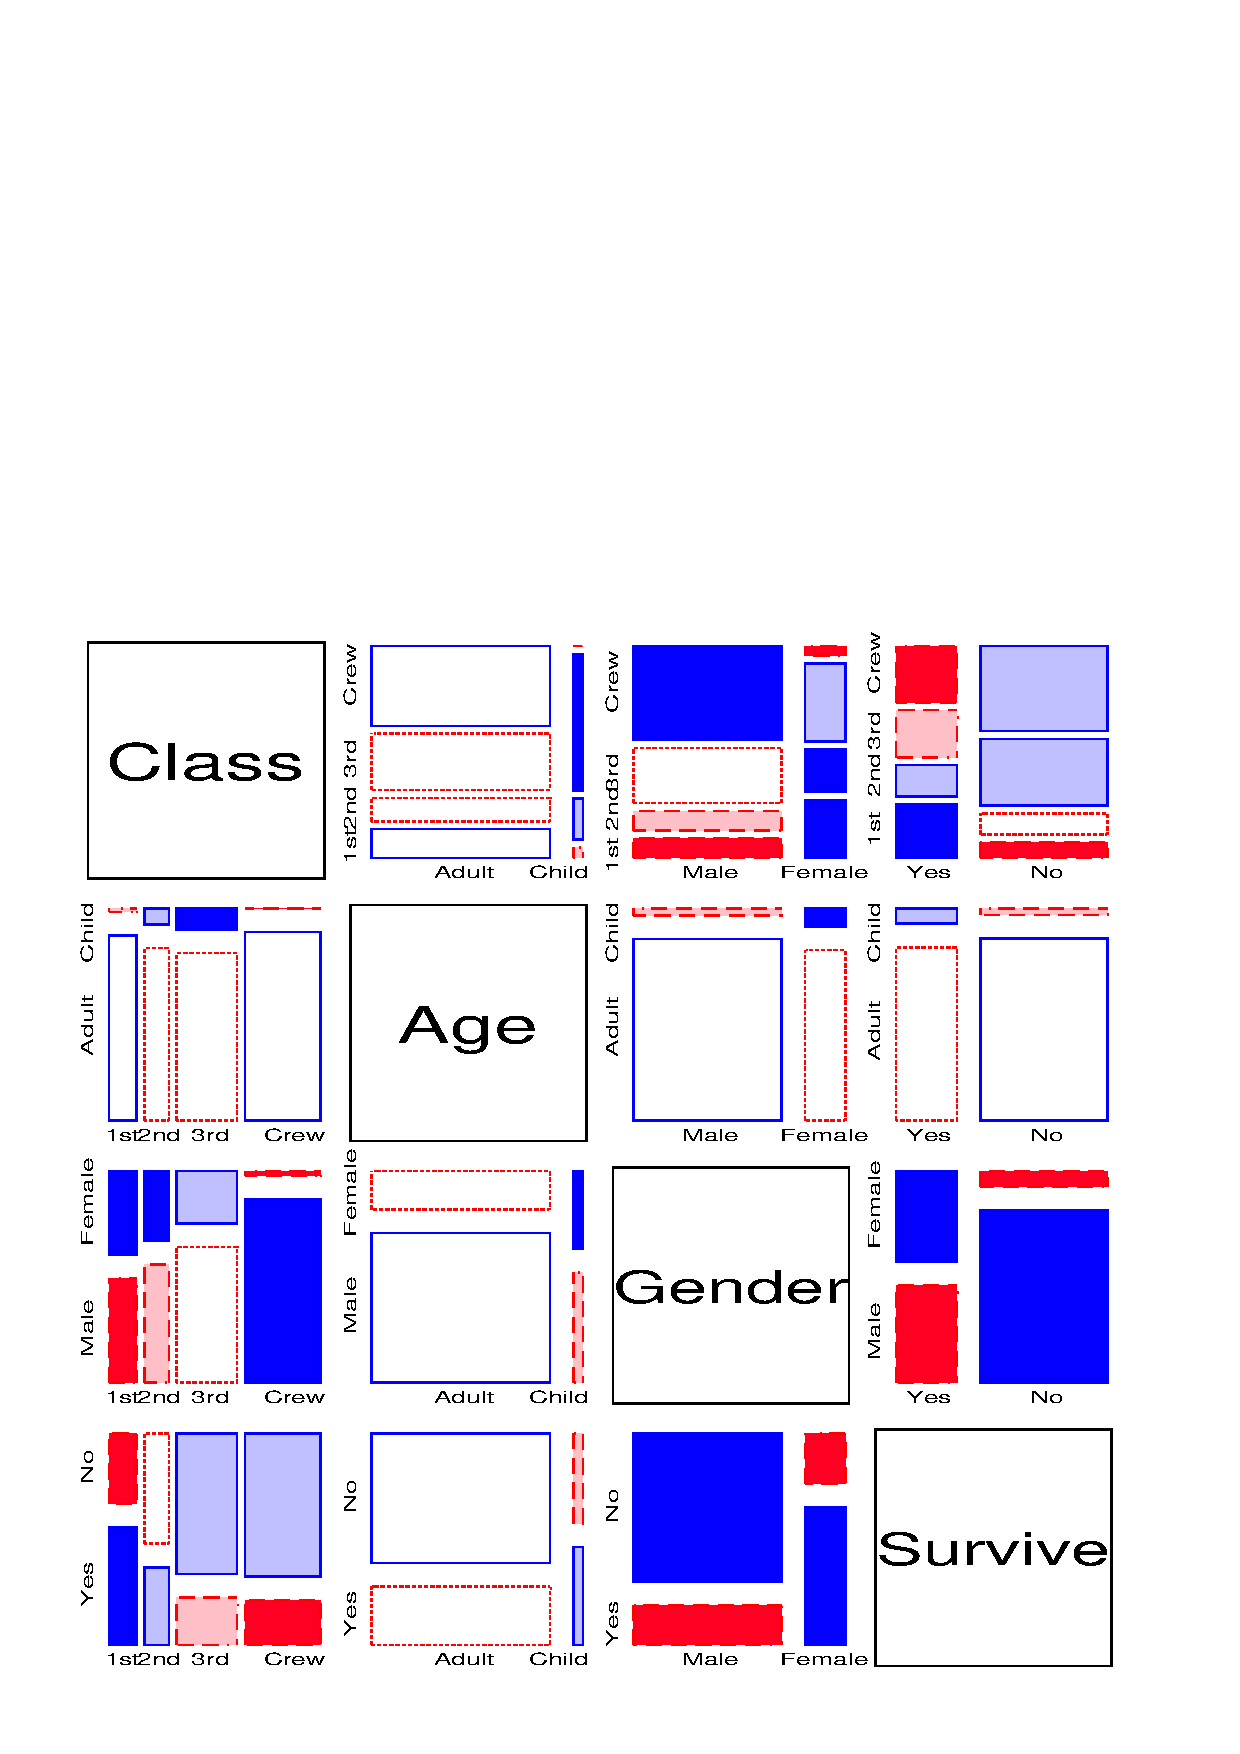
\includegraphics[scale=.7]{ch5/fig/titanmos}
  \caption[Mosaic matrix of \emph{Titanic} data]{Mosaic matrix of \emph{Titanic} data.  Each panel shows the marginal relation,
fitting an independence model between the row and column variable, collapsed over other variables.}\label{fig:titanmos}
\end{figure}
\end{Example}

\begin{Example}[marital3]{Marital status and pre- and extramarital sex}
The data on the relation between marital status and reported
premarital and extramarital sex was explored earlier using mosaic
displays in \exref{ex:marital1} and \exref{ex:marital2}.

The $2\times 2 \times 2 \times 2$ table in frequency form can be
analyzed as shown below, where the classification variables are
\pname{GENDER}, \pname{PRE}, \pname{EXTRA}, and \pname{MARITAL}.

\begin{listing}
data marital;
   input gender $ pre $ extra $ @;
    pre = 'Pre:' || pre;
    extra = 'X:' || extra;
   marital='Divorced';  input freq @;  output;
   marital='Married';   input freq @;  output;
datalines;
Women  Yes  Yes   17   4
Women  Yes  No    54  25
Women  No   Yes   36   4
Women  No   No   214 322
Men    Yes  Yes   28  11
Men    Yes  No    60  42
Men    No   Yes   17   4
Men    No   No    68 130
;

proc corresp data=marital mca outc=coords;
    weight freq;
    tables gender pre extra marital;
run;
\end{listing}
The same analysis, with the addition of the 2D plot of
category scores, would be produced by the \macro{CORRESP},
\begin{listing}
%corresp(data=marital, tables=gender pre extra marital, weight=freq, 
   options=mca short, interp=vec, inc=1, pos=-, symbols=dot);
\end{listing}

\begin{Output}[htb]
\caption{Chi-Square Decomposition for Marital status MCA}\label{out:maritalmca1}
\begin{output}
                      Inertia and Chi-Square Decomposition

        Singular  Principal Chi-                                        
        Values    Inertias  Squares Percents    8   16   24   32   40   
                                            ----+----+----+----+----+---
        0.62226   0.38721   1796.45  38.72% ************************    
        0.50915   0.25923   1202.70  25.92% ****************            
        0.43375   0.18814    872.86  18.81% ************                
        0.40672   0.16542    767.47  16.54% **********                  
                  -------   -------                                     
                  1.00000   4639.48 (Degrees of Freedom = 49)           
\end{output}
\end{Output}
%% one figure
\begin{figure}[htb]
  \centering
  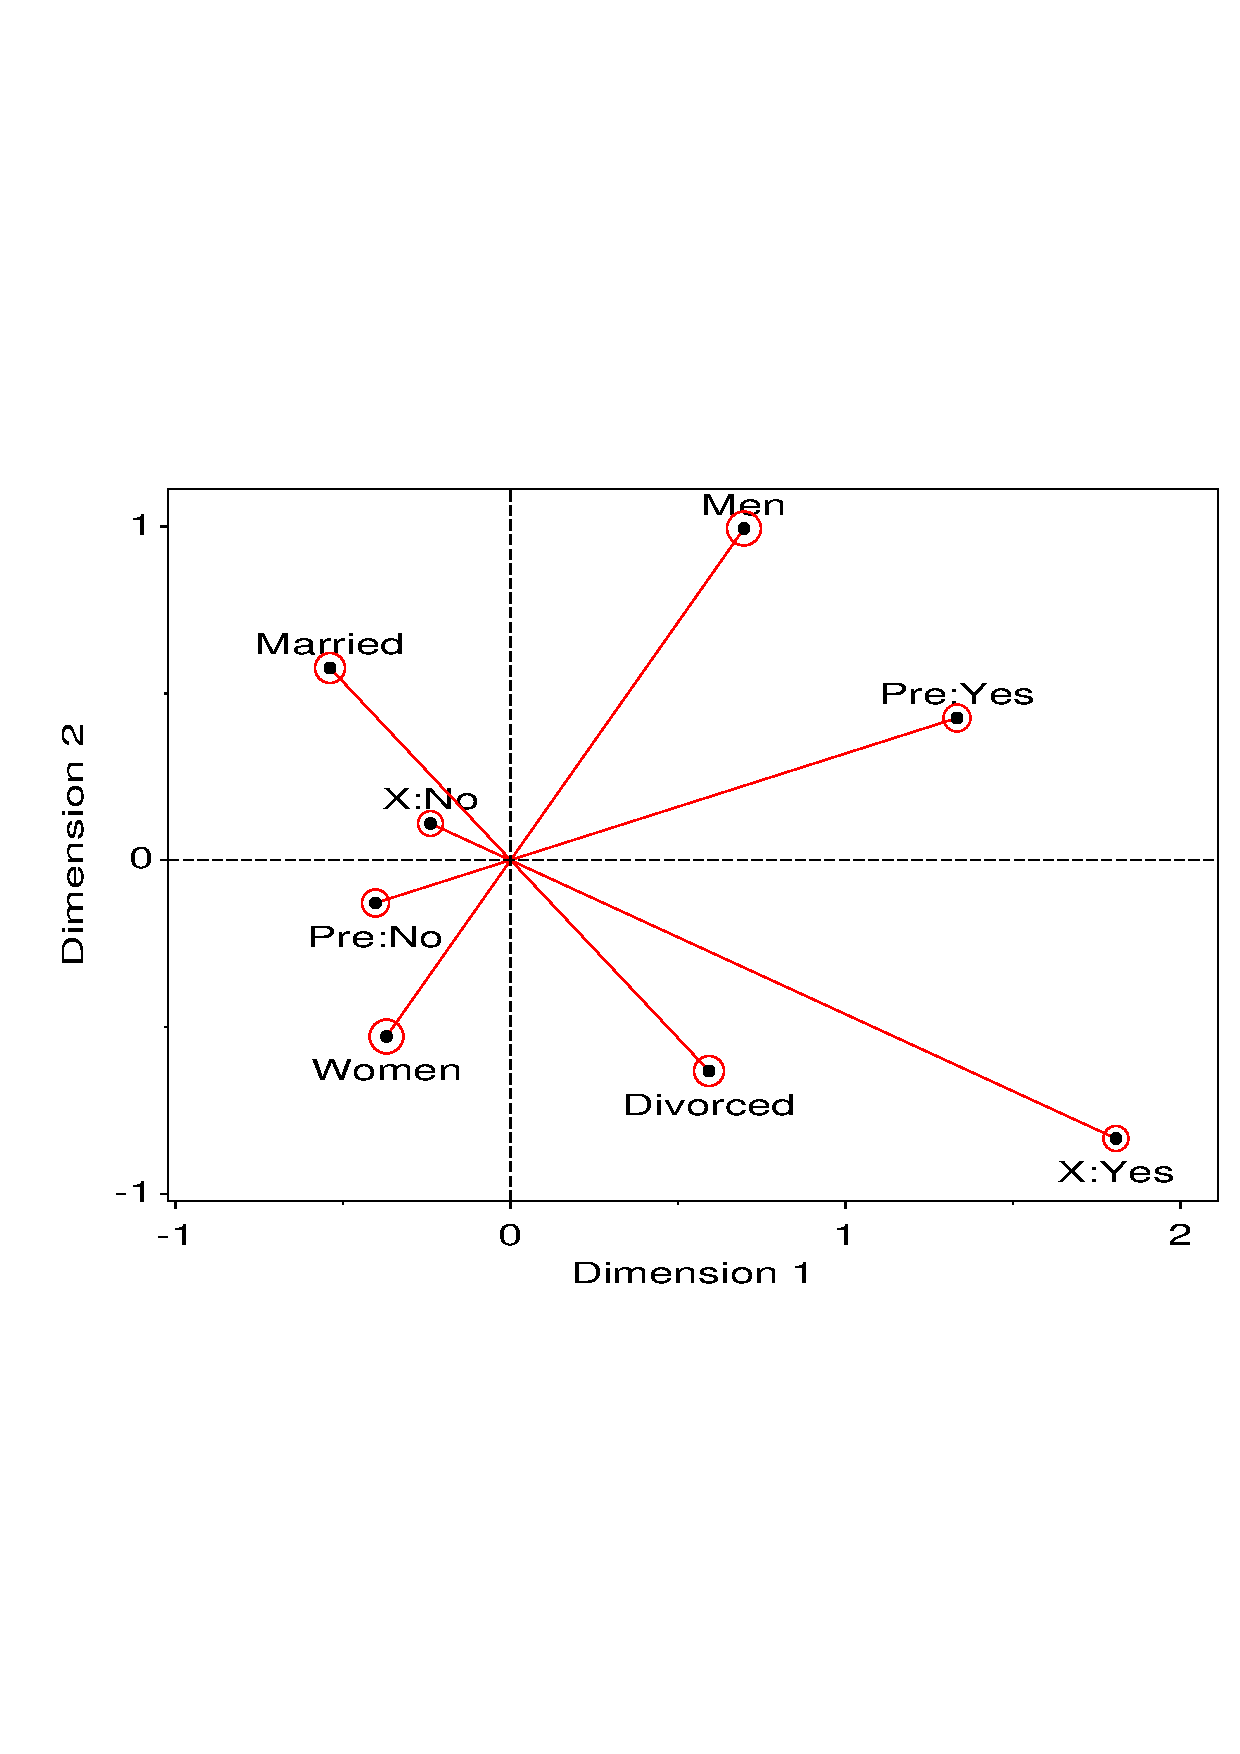
\includegraphics[scale=.8,clip]{ch5/fig/mcamarital1}
  \caption{2D multiple \CA\ display for marital status data}%
  \label{fig:mcamarital1}
\end{figure}

An enhanced version%
\footnote{The size of the bubble symbol surrounding each point is proportional
to the quality of the representation in two dimensions.}
of this plot is shown in \figref{fig:mcamarital1}.
The principal inertias, listed in \outref{out:maritalmca1}, again suggest
that two dimensions are sufficient for this \Dset.
The positions of the category points on Dimension 1 suggest that Women
are less likely to have had pre-marital and extra-marital sex
and that still being married is associated with the absence of pre- and extra-marital sex.

Although two dimensions are probably sufficient for interpreting these
data, we illustrate three-dimensional plots briefly.
When you specify the parameter \pname{DIM=3},
the \macro{CORRESP} produces a coordinates \Dset\ and an \ADS\
with three dimensions.%
\footnote{The first two dimensions are identical to the 2D solution,
because of the nested nature of CA and MCA solutions.}
It also produces a labeled \PROC{G3D} scatter plot.
However, the \pname{G3D} procedure does not allow axes to be equated,
and it is usually necessary to experiment with the \pname{ROTATE}
and \pname{TILT} options to produce a reasonable display, so the plot
generated by the macro should be considered just a first approximation.

A three-dimensional MCA solution for the Marital status data is produced with
this statement:
%% input: /Users/friendly/sasuser/catdata/mcamar.sas
%% last modified: 24-Jul-99 15:56
\begin{listing}
%corresp(data=marital, tables=gender pre extra marital, weight=freq, dim=3, 
   plotreq=dim1 * dim2 = dim3,
   options=mca short, interp=vec, symbols=dot,
   out=coord, anno=label);
\end{listing}
  

To roughly equate the axes,
the initial plot (not shown) was modified by extending the plotting range
for all dimensions as shown below.   Some additional annotation steps
(not shown) produces \figref{fig:mcamarital2}.  Note that the projections
of the points on the Dim1--Dim2 plane is identical to the solution shown
in \figref{fig:mcamarital1}.
%% input: /Users/friendly/sasuser/catdata/mcamar.sas
%% last modified: 21-Jul-99 11:19
\begin{listing}
data xtra;              /* Add dummy points to extend X, Y range */
   input dim1-dim3 shapevar $;
datalines;
 2   1  -.6  POINT
-1  -1  -.6  POINT
data coord;
   Set coord xtra;

goptions vsize=6in hsize=8in;
proc g3d data=coord;
   scatter dim1 * dim2 = dim3
      / shape='point' color='green'
        zmin=-0.6 tilt=80 rotate=75 caxis=gray60
        xticknum=2 yticknum=2 zticknum=2 grid
        annotate=label;
\end{listing}
  
\begin{figure}[htb]
  \centering
  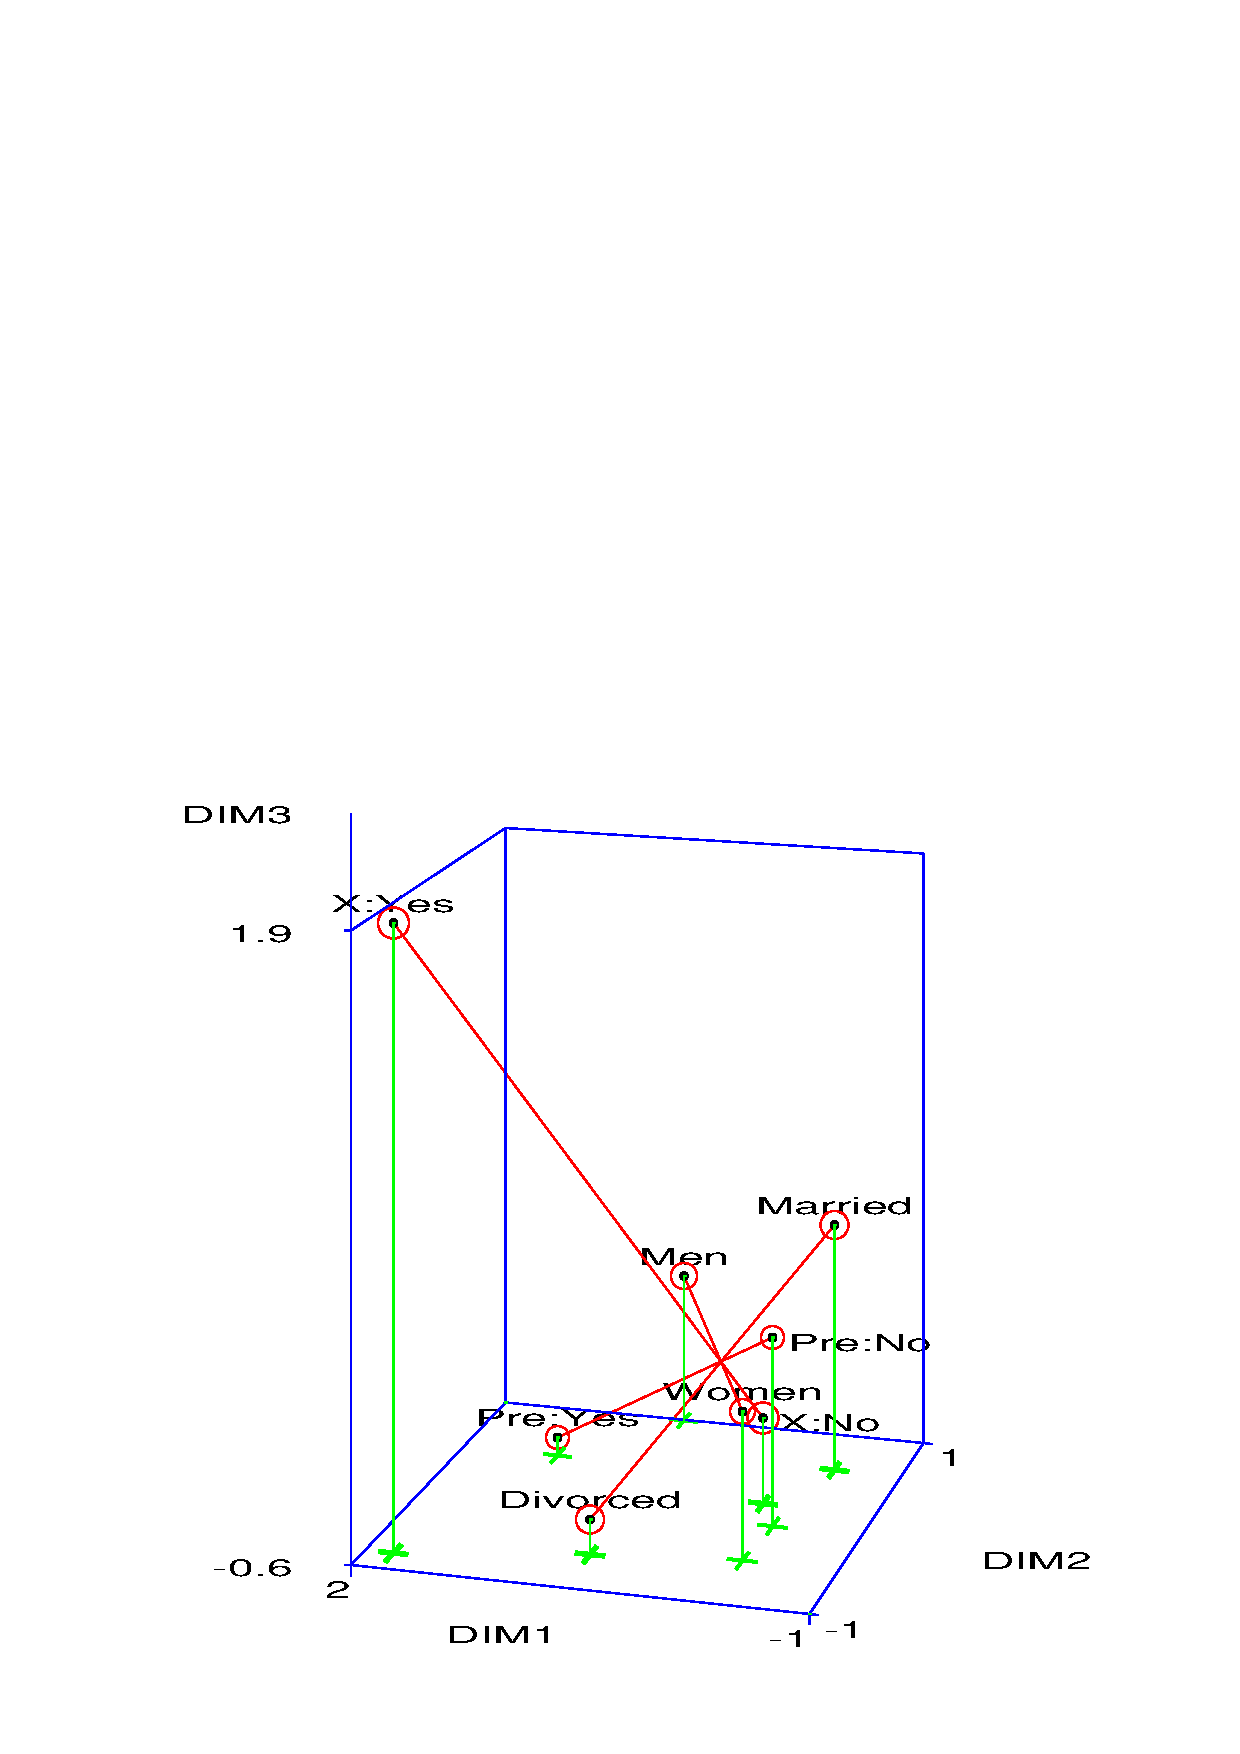
\includegraphics[scale=.8,clip]{ch5/fig/mcamarital2}
  \caption{3D multiple \CA\ display for marital status data}%
  \label{fig:mcamarital2}
\end{figure}
\end{Example}

\section{Extended MCA: Showing interactions in $2^Q$ tables}\label{sec:ca-mcainter}
\ixon{multiple correspondence analysis!extended}
As we discussed earlier,
MCA was developed as a way to depict the relationships among the
categories of multiple categorical variables, and the derivation of
the method based on the Burt matrix implies that only the relations
in the bivariate marginal tables are represented in the displays.
\ix{Burt matrix}
This is based on the assumption \citep{Gifi:90,Greenacre:88}
that, as with multivariate normal data, the structural relations
among variables are adequately captured by bivariate associations.%
\footnote{Another concern is that higher-way \ctab s may become
sparse, hence resulting in instability in solutions
\citep{Heijden:87}.}
These developments, and usually practice, have led to the mistaken beliefs that,
\begin{seriate}
\item MCA can \emph{only}
represent bivariate (first-order) interactions,
\item MCA can \emph{only} portray the category points of the variables
(not their combinations), and
\item associations must be inferred from the relative positions of
the category points.
\end{seriate}

A recent paper by \citet{MeulmanHeiser:97} demonstrates, however,
that none of these are necessary consequences of MCA itself.
Moreover, for the case of binary variables (a $2^Q$ table),
an odds interpretation of distances between category points
leads to simple geometrical patterns in MCA plots.

Their method for including higher-order effects involves adding all cross-terms,
up to a given order,
to the set of variables in frequency form which are analyzed by
MCA.  For example, with three variables, $A$, $B$, and $C$,
generate all interaction terms (using the \texttt{|} syntax of
\PROC{GLM} or \PROC{CATMOD}),
\begin{equation*}
\mbox{\texttt{A | B | C}} \iff \mbox{\texttt{A B C A*B A*C B*C A*B*C}}
\end{equation*}
\begin{table}[htb]
 \caption[Extended factor matrix for a $2\times 2\times2$ table]%
         {Extended factor matrix for a $2\times 2\times2$ table, including all possible cross-classifications.}\label{tab:mcadesign}\vspace{5pt}
\begin{center}
\begin{tabular}{lll | ccc ccc c}
 \hline
       &       &        &  A  &  B  &  C  &  AB &  AC &  BC & ABC \\ \hline
 $a_1$ & $b_1$ & $c_1$  &  1  &  1  &  1  &  1  &  1  &  1  &  1 \\
       &       & $c_2$  &  1  &  1  &  2  &  1  &  2  &  2  &  2 \\
       & $b_2$ & $c_1$  &  1  &  2  &  1  &  2  &  1  &  3  &  3 \\
       &       & $c_2$  &  1  &  2  &  2  &  2  &  2  &  4  &  4 \\
%
 $a_2$ & $b_1$ & $c_1$  &  2  &  1  &  1  &  3  &  3  &  1  &  5 \\
       &       & $c_2$  &  2  &  1  &  2  &  3  &  4  &  2  &  6 \\
       & $b_2$ & $c_1$  &  2  &  2  &  1  &  4  &  3  &  3  &  7 \\
       &       & $c_2$  &  2  &  2  &  2  &  4  &  4  &  4  &  8 \\
%
\end{tabular}
\end{center}
\end{table}

Similarly, the \texttt{@} syntax specifies all terms up to a given
order; for example,
\begin{equation*}
\mbox{\texttt{A | B | C | D}@2} \iff \mbox{\texttt{A B C D A*B A*C A*D B*C B*D C*D}}
\end{equation*}
generates all
terms up to order 2.  To illustrate, \tabref{tab:mcadesign} shows all terms
for the three-way model \texttt{(A | B | C)}.
Like any \pname{CLASS} variables, it is only necessary for the variable
values to be discrete.
However, it is strictly necessary to include \emph{all} terms at the same
interaction level, up to the given order.

The indicator matrix will then consist of the dummy variables for
these terms, so that, for \tabref{tab:mcadesign},
$\mat{Z} = [
 \mat{Z}_A  \mat{Z}_B  \mat{Z}_C  \mat{Z}_{AB}
 \mat{Z}_{AC}  \mat{Z}_{BC}  \mat{Z}_{ABC}
]$.
Forming the Burt matrix, $ \mat{B} =  \mat{Z}\trans  \mat{Z}$,
we see that the off-diagonal blocks now contain \emph{all}
contingency tables which can be formed from the original variables
(up to the specified order), not just the pairwise bivariate
tables.
The category points for an MCA solution based on this
extended $\mat{Z}$ matrix will then contain, in addition to the
usual one-way ``main effect'' points
of the variables themselves, sets of interaction points
(e.g., $(ab)_{ij}$, $(ac)_{ik}$, and so forth) for the various
combinations of factors included.

What happens to the category points for these interaction terms in the MCA
solution?
\citet{MeulmanHeiser:97} demonstrate the remarkable results that
\begin{itemize*}
\item distance ratios between sets of interaction points correspond to
odds ratios in the higher-order table,
and
\item the various independence structures we have considered
(cf. \tabref{tab:hyp3way})
give rise to simple configurations of points in the category
space.
\end{itemize*}

For simplicity, consider a $2\times 2$ table with cell probabilities
$p_{ij}$.  Let $\vec{z}_{ij}$
refer to the profile coordinate points for the $(ab)_{ij}$
combinations, and let $\vec{z}_{i\bullet}$, $\vec{z}_{\bullet j}$
be the coordinate points for the one-way $A$ and $B$ effects,
respectively.  Then, the  $\vec{z}_{ij}$ define a quadrilateral,
and the $\vec{z}_{i\bullet}$ and $\vec{z}_{\bullet j}$ are the
centroids (weighted by $p_{ij}$) of the corresponding corners,
as shown in \figref{fig:mcaidemo}.  In this figure, the mass, $p_{ij}$ of each cell point is indicated by its size and the $z$ points are labeled
by their subscripts.

\begin{figure}[htb]
  \centering
  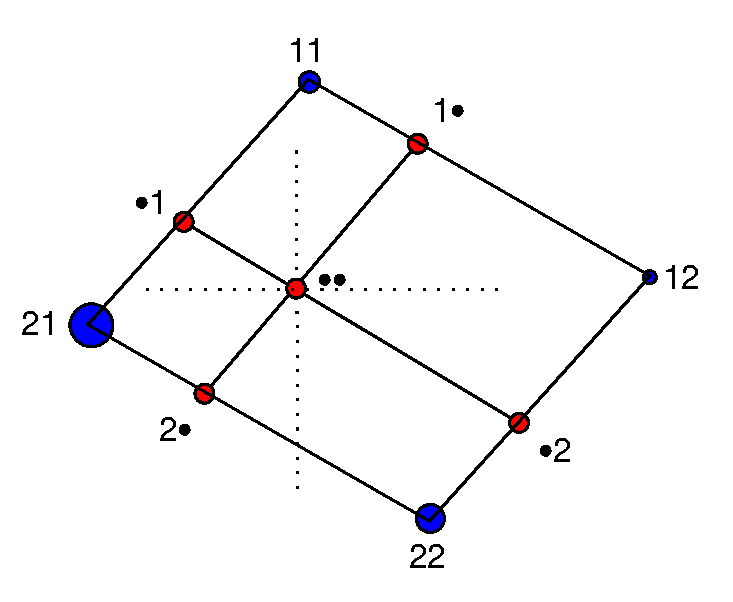
\includegraphics[scale=.9,clip]{ch5/fig/mcaidemo}
  \caption[Category points and profile points in extended MCA representation]{Category points ($\vec{z}_{ij}$) and profile points
  ($\vec{z}_{i\bullet}$, $\vec{z}_{\bullet j}$) in extended MCA representation. Under independence, the lines connecting the profile points are parallel to those connecting corresponding category points.}\label{fig:mcaidemo}
\end{figure}
The centroid points are related to the interaction points as (weighted)
linear combinations:
\begin{eqnarray*}%\label{eq:mcainter1}
  \vec{z}_{i \bullet} & = &
   \frac{p_{i1}}{p_{i+}} \: \vec{z}_{i1} +
   \frac{p_{i2}}{p_{i+}} \: \vec{z}_{i2} \\
  \vec{z}_{\bullet j} & = &
   \frac{p_{1j}}{p_{+j}} \: \vec{z}_{1j} +
   \frac{p_{2j}}{p_{+j}} \: \vec{z}_{2j}
\end{eqnarray*}
Now, for any edge of the quadrilateral, e.g., $z_{i1}$, $z_{i2}$,
their centroid is located on the line between them, so the
distances must be additive,
\begin{equation*}%\label{eq:mcainter2}
  d( \vec{z}_{i1}, \vec{z}_{i2} ) =
  d( \vec{z}_{i1}, \vec{z}_{i \bullet} ) +
  d( \vec{z}_{i \bullet}, \vec{z}_{i2} )
\end{equation*}
From these relations, \citet{MeulmanHeiser:97} show that:
\begin{itemize}
\item Given $A=i$ (or, $B=j$), the odds of being in category 1 vs. category 2
of $B$ (or $A$) are shown in the display by the inverse ratio of their
distances to their centroid.  For example,
\begin{equation*}%\label{eq:mcainter3}
  \frac{p_{i1}}{p_{i2}} =
  \frac{ d( \vec{z}_{i2}, \vec{z}_{i \bullet} ) }
       { d( \vec{z}_{i1}, \vec{z}_{i \bullet} ) }
\end{equation*}
\item The odds ratio $\theta$ has a simple multiplicative relation
to these distances among the four corner points and their
centroids.
\begin{equation}\label{eq:mcainter4}
  \theta =
  \frac{p_{11} p_{22}}{p_{12} p_{21}} =
  \frac{ d( \vec{z}_{12}, \vec{z}_{\bullet 2}) \: d( \vec{z}_{21}, \vec{z}_{\bullet 1} )}
       { d( \vec{z}_{11}, \vec{z}_{\bullet 1}) \: d( \vec{z}_{22}, \vec{z}_{\bullet 2} )}
\end{equation}
\item Under independence, $\theta =1$, and \eqref{eq:mcainter4}
therefore implies that
(a) the corner points form a parallelogram, and
(b) the lines connecting the centroids of the same variable
(e.g., $(\vec{z}_{\bullet 1}, \vec{z}_{\bullet 2}))$ are parallel
to those of their respective category points.
These relations of parallelism and additivity are shown in \figref{fig:mcaidemo}.
\end{itemize}

Although this discussion was presented
in terms of a $2 \times 2$ table, the geometrical relations extend
directly to \emph{any} number of binary variables.
For a $2 \times 2 \times 2$ table,  the models of various types of
independence shown in \tabref{tab:hyp3way} can all be characterized
in terms of the three odds ratios for all pairs of variables, and
therefore in terms of parallelism and additivity of the corresponding
pairwise quadrilaterals in the spatial representation.
Essentially, each independence relation corresponds to one odds ratio $\theta=1$,
which in turn is shown as one two-way term whose profile points form
a parallelogram, as shown in the table below.
 \begin{center}
 \begin{tabular}{lll c}
 \hline
            &  Independence  &             &  Number of parallel    \\
Hypothesis  &  relations     & Odds ratios &  two-way profile sets  \\ \hline
$H_1$  & $A \perp B \perp C$ &  $\theta_{AB} = \theta_{AC} = \theta_{BC} = 1$ & 3 \\
%
$H_2$  & $A , B \perp C$     &  $\theta_{AC} = \theta_{BC} = 1$ & 2 \\
%
$H_3$  & $A \perp B \given C$ &  $\theta_{AB} = 1$               & 1 \\
%
$H_4$  & none                & all $\theta \neq 1$               & 0 \\
%
  \hline
 \end{tabular}
 \end{center}


The following example demonstrates these ideas with a $2^3$ table, where
one two-way term is independent by design.
It also illustrates how to generate the interaction
variables, and some special techniques for displaying the extended
MCA solution.

\begin{Example}[bartlett]{Bartlett's data}
In a classic paper that extended the notion of interaction to three-way
tables, \citet{Bartlett:35} gave the data shown in \tabref{tab:bartlett}
from an experiment designed to investigate the propagation of
plum root stocks from cuttings.
In the $2 \times 2 \times 2$ table, time of planting (T) and length
of cutting (L) are factors; whether the cutting was alive or dead (A)
was the response.
Note that the column totals for the factors are all equal,
these having been fixed by the experimental design.
Thus, there can be
no $T\times L$ marginal association, and interest naturally is focused
on the [AT] and [AL] associations.
%%
%% Table bartlett written by md2tex 13AUG98 12:17
%%
\begin{table}[htb]
 \caption{Bartlett's data on propagation of plum root stocks}
 \label{tab:bartlett}
 \begin{center}
  \begin{tabular}{|l|rrrr|r|}
   \hline
 & \multicolumn{4}{c|}{\bfseries\large Time of planting} & \rule{0in}{2.5ex}\\
 & \multicolumn{2}{c|}{Now   } & \multicolumn{2}{c|}{Spring} &  \\\cline{2-5}
 & \multicolumn{4}{c|}{\bfseries\large Length of cutting} & \rule{0in}{2.5ex}\\
{\bfseries\large Alive?} & Long   & Short  & Long   & Short & {\bfseries\large Total} \\
   \hline
Alive    &      156 &      107 &       84 &       31 &      378 \\
Dead     &       84 &      133 &      156 &      209 &      582 \\
   \hline
\rule{0in}{2.5ex}{\bfseries\large Total} &     240 &      240 &      240 &      240 &      960 \\
   \hline
  \end{tabular}
 \end{center}
\end{table}


The marginal relations are easily seen in a mosaic matrix, shown in
\figref{fig:mosmat1m}. Time and Length are independent, but
there is a strong [AT] association, with planting
now more likely to be successful, and a weaker [AL] association,
so that long cutting are more likely to survive.

\begin{figure}[htb]
  \centering
  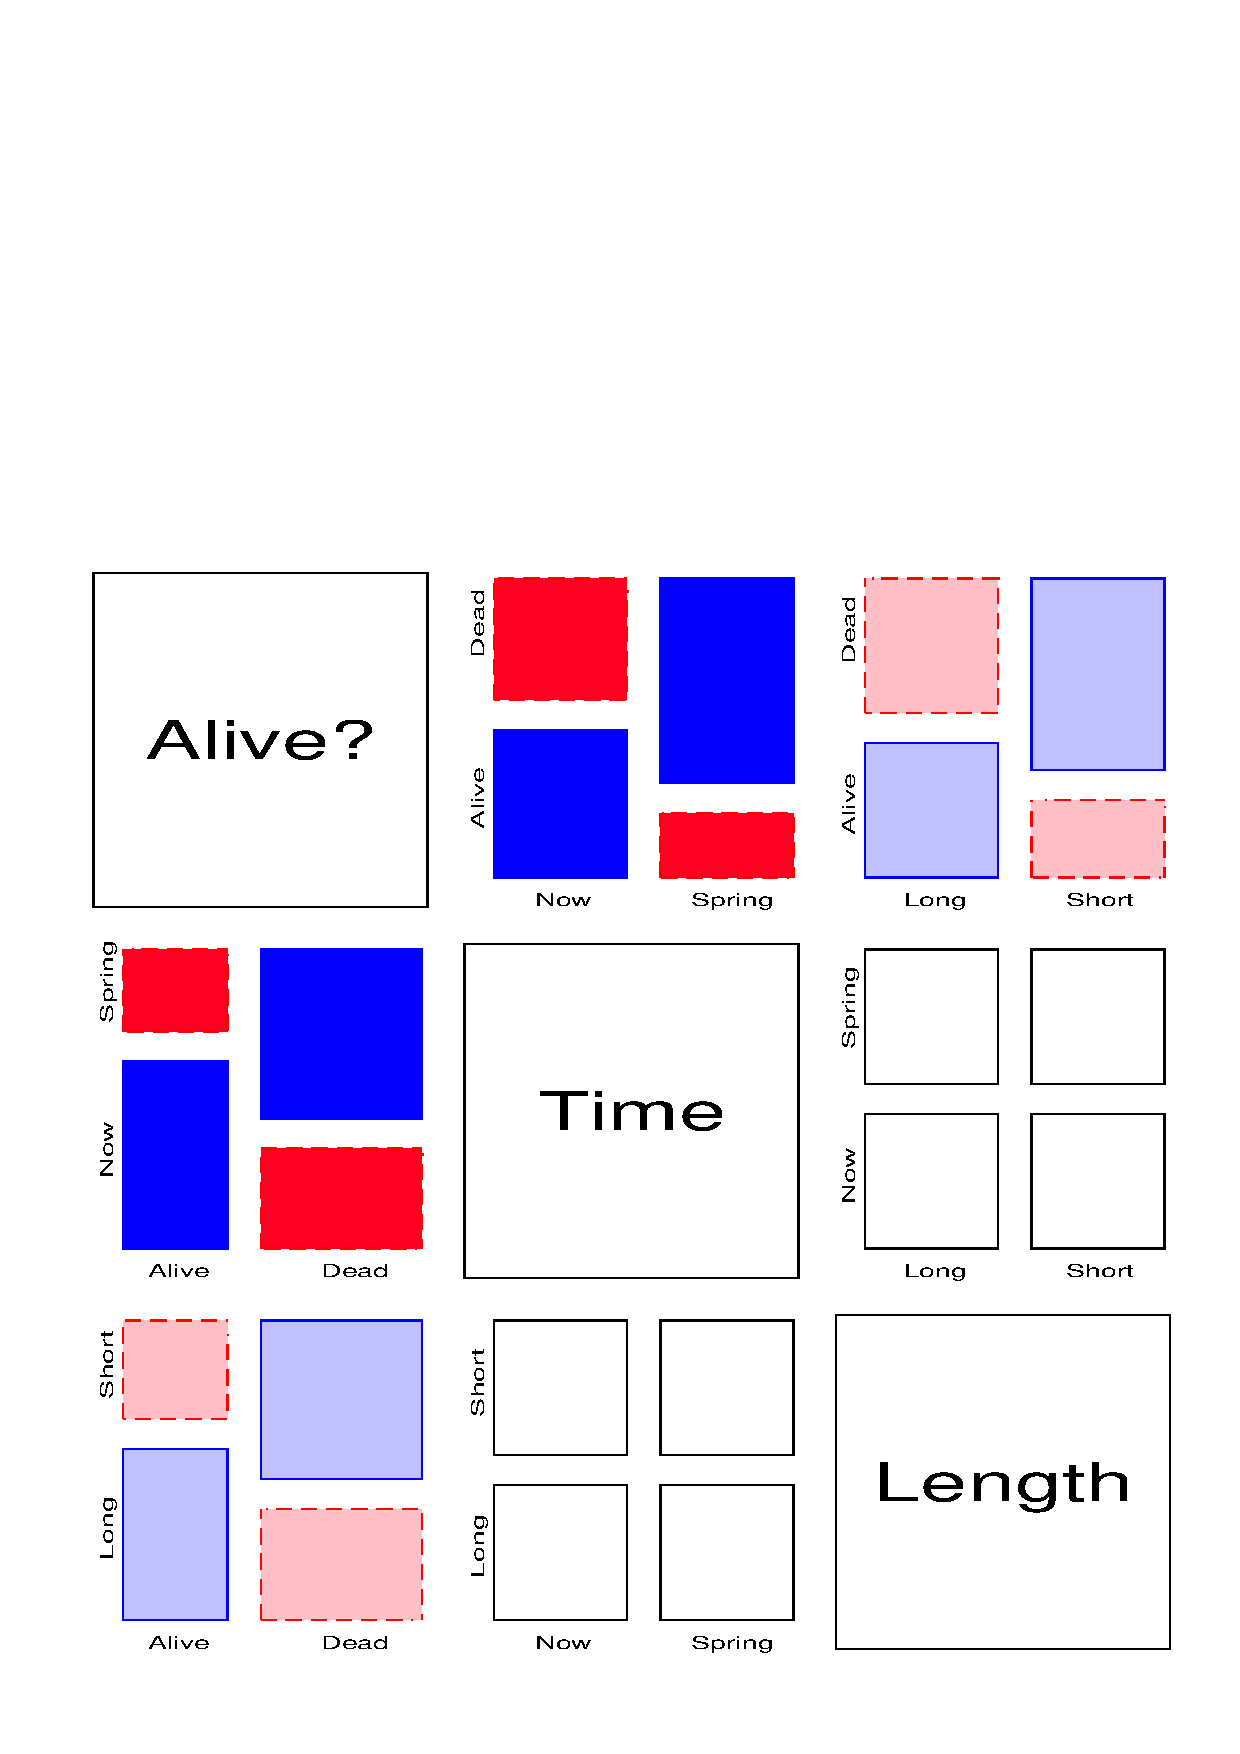
\includegraphics[scale=.7,clip]{ch5/fig/mosmat1m}
  \caption{Mosaic matrix for marginal associations in Bartlett's data}\label{fig:mosmat1m}
\end{figure}
The standard MCA analysis is carried out with the statements below.
In the call to the \macro{CORRESP}, the \mparm{INTERP=VEC}{CORRESP}
draws vectors from the origin to each main category point.
The macro produces the graph of the 2D solution shown in \figref{fig:mcabart1}; the principal inertias are shown in
\outref{out:mcabart1}.
%% input: /Users/friendly/sasuser/catdata/mcabart.sas
%% last modified: 26-Jul-99 10:48
\begin{listing}
data bartlett;
   do alive='Alive', 'Dead';
      do time='Now   ', 'Spring';
         do Length = 'Long ', 'Short';
            input count @;
            output;
            end;
         end;
      end;
datalines;
 156 107  84  31
  84 133 156 209
;
*-- Ordinary MCA of the three variables;
%corresp(data=bartlett, tables=Alive Time Length, weight=count,
   options=mca short, interp=vec, inc=0.2, pos=-,
   symbols=dot, colors=black, m0=0);
\end{listing}


\begin{figure}[htb]
  \centering
  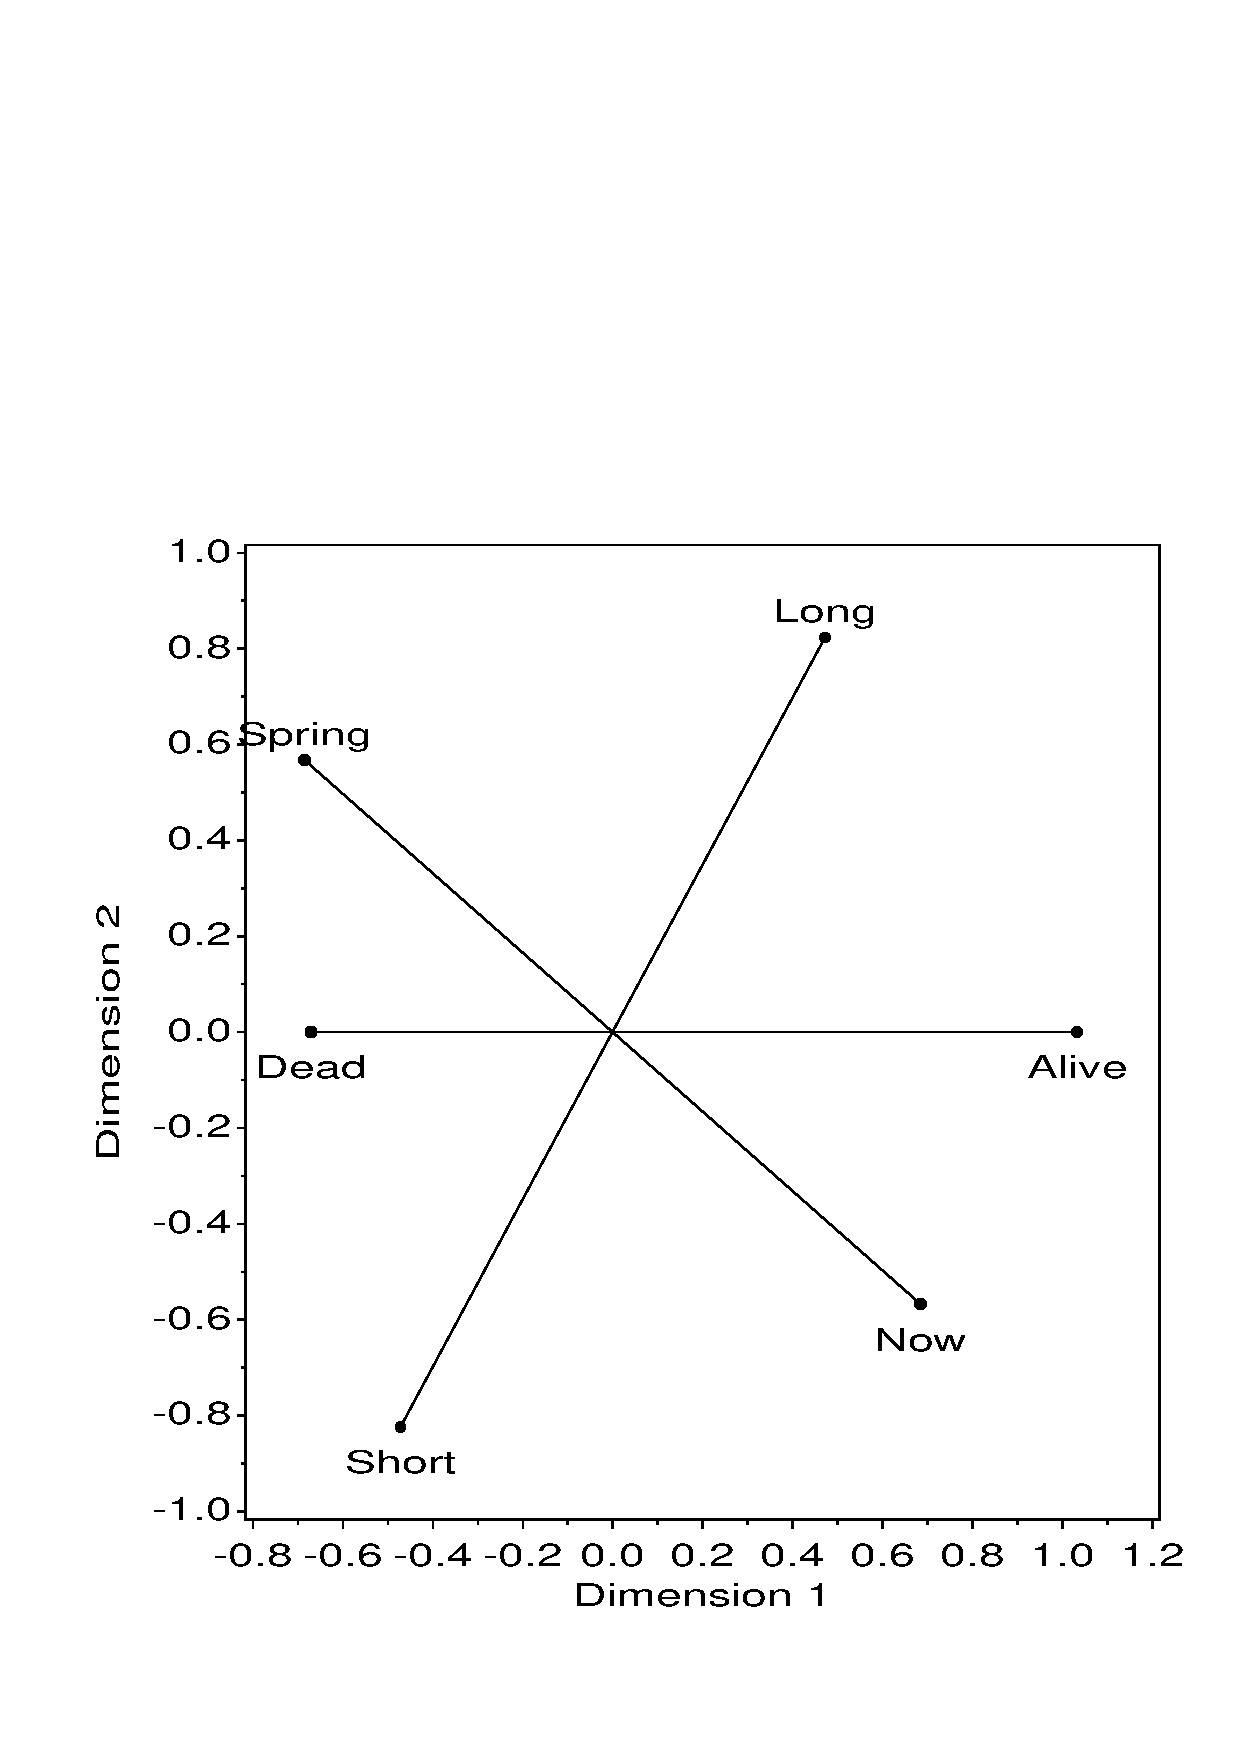
\includegraphics[scale=.7,clip]{ch5/fig/mcabart1}
  \caption{2D MCA solution for Bartlett's data}\label{fig:mcabart1}
\end{figure}

The interpretation of \figref{fig:mcabart1} is quite simple.
Dimension 1 is perfectly aligned with the Alive response variable.
The associations [AT] and [AL] of Time and Length are shown by their projections
(coordinates) on this axis.
Time has a stronger association, so its projection on this axis is larger,
and planting Long cuttings, Now leads to increased survival.
The independence of Time and Length is shown by the nearly
right angle between their vectors.%
\footnote{In an equated 3D representation, they \emph{are} orthogonal.}
Because the second principal inertia in \outref{out:mcabart1}
equals $1/Q = 1/3$ we do not interpret the second dimension.
\begin{Output}[htb]
\caption{Chi-Square Decomposition for Bartlett's data, MCA}\label{out:mcabart1}
\begin{output}
                      Inertia and Chi-Square Decomposition

        Singular  Principal Chi-
        Values    Inertias  Squares Percents    9   18   27   36   45
                                            ----+----+----+----+----+---
        0.67902   0.46107   1457.90  46.11% **************************
        0.57735   0.33333   1053.99  33.33% *******************
        0.45342   0.20559    650.08  20.56% ***********
                  -------   -------
                  1.00000   3161.97 (Degrees of Freedom = 25)
\end{output}
\end{Output}
Note also how the odds are shown by distance ratios in the plot.
Both Time and Length have equal marginal frequencies for their two
levels (odds = 1), and the ratio of distances to the origin for
the levels of both variables equals 1.0.
The ratio of distances to the origin for Alive and Dead
is inversely related to their marginal frequencies.

The statements below illustrate one way to construct the interaction
variables representing the first-order associations [AT], [AL], and [TL]
and the second-order interaction, [ATL].
Each of the character variables \pname{ALIVE}, \pname{TIME},
and \pname{LENGTH} is used to create a dummy (0/1) variable
(\pname{A}, \pname{T}, and \pname{L}, respectively).
The interaction terms are then created with binary arithmetic
in the \Dstp\ \pname{COMBO}.
A \PROC{FORMAT} step is used to create short character labels for the
combinations, to be used in the plots which follow.
These labels use an upper case letter to refer to the first level of
each main variable and a lower case letter to refer to the second level.

The \Dset\ \pname{COMBO} which results is shown in \outref{out:mcabart2}.
Note that the variables \pname{A--ATL} are actually numeric, but are printed
using their formatted values.%
\footnote{Because the interaction
variables need only be discrete, they could be created more easily, simply
by concatenating the main variables,
(e.g., \texttt{AT = ALIVE || TIME;}, and so forth).  This would produce
cluttered displays, however, because each combination is plotted and labeled.}
%
%% input: /users/faculty/friendly/sasuser/catdata/mcabart.sas
%% last modified: 13-Aug-98 17:34
\begin{listing}
*-- Formats for higher-order effects;
proc format;
   value a  0='a' 1='A';
   value t  0='t' 1='T';
   value l  0='l' 1='L';
   
   value at 0='at' 1='aT' 2='At' 3='AT';
   value al 0='al' 1='aL' 2='Al' 3='AL';
   value tl 0='tl' 1='tL' 2='Tl' 3='TL';
   value atl 0='atl' 1='atL' 2='aTl' 3='aTL' 4='Atl' 5='AtL' 6='ATl' 7='ATL';

*-- Code combinations of variables;
data combo;
   set bartlett;
   
   a = (alive='Alive');
   t = (time='Now');
   l = (length='Long');
   
   at = 2*a + t;
   al = 2*a + l;
   tl = 2*t + l;
   
   atl = 4*a + 2*t + l;
   format a a. t t. l l.  at at.  al al.  tl tl.  atl atl.;
proc print noobs;

\end{listing}

\begin{Output}[htb]
\caption{\Dset\ \pname{COMBO}: Interactive coding for Bartlett's data, Extended MCA}\label{out:mcabart2}
\begin{output}
   LENGTH    TIME      ALIVE    COUNT    A    T    L    AT    AL    TL    ATL

   Long      Now       Alive     156     A    T    L    AT    AL    TL    ATL
   Long      Now       Dead       84     a    T    L    aT    aL    TL    aTL
   Long      Spring    Alive      84     A    t    L    At    AL    tL    AtL
   Long      Spring    Dead      156     a    t    L    at    aL    tL    atL
   Short     Now       Alive     107     A    T    l    AT    Al    Tl    ATl
   Short     Now       Dead      133     a    T    l    aT    al    Tl    aTl
   Short     Spring    Alive      31     A    t    l    At    Al    tl    Atl
   Short     Spring    Dead      209     a    t    l    at    al    tl    atl
\end{output}
\end{Output}

Applying MCA to this \Dset\ using the main effect variables \pname{A T L}
would produce results identical to \figref{fig:mcabart1}.
Adding the three two-way variables, \pname{AT AL TL} will add $3 \times 4$
category points for the pairwise combinations of these factors.
The three-way variable, \pname{ATL}, adds an additional
8 category points, representing the individual cells in the table.

The analysis shown below excludes the three-way \pname{ATL} terms for simplicity.
As long as the terms are added in a balanced way
(including all terms of a given order), the positions of points tend to be very
similar whether or not terms of higher-order are included.

%% input: /users/faculty/friendly/sasuser/catdata/mcabart.sas
%% last modified: 16-Aug-98 12:26
\begin{listing}
proc corresp data=combo  mca outc=coords short;
   weight count;
   tables a t l at al tl;* atl;

*-- Identify the size and name of each effect;
data coords;
   set coords;
   where (_type_) = 'VAR';
   drop _type_ inertia contr1--best;
   terms=length(_name_);
   effect = upcase(_name_);
   label dim1 = 'Dimension 1'
         dim2 = 'Dimension 2';
proc sort;
   by terms effect _name_;
proc print;
   id _name_ effect terms;
   var dim1 dim2 mass;
\end{listing}

The \ODS\ \pname{COORDS} is used to produce the plots
shown in \figref{fig:mcabart2}.
In order to draw the vectors for the main effect points,
and quadrilaterals for the two-way terms
as in \figref{fig:mcaidemo}, variables \pname{TERMS} and \pname{EFFECT}
are added to the \pname{COORDS} \Dset\ as shown above.

%% two subfig side-by-side
\begin{figure}[htb]
 \begin{minipage}[t]{.49\linewidth}
  \includegraphics[width=1\linewidth]{ch5/fig/mcabart2}
 \end{minipage}%
 \hfill
 \begin{minipage}[t]{.49\linewidth}
  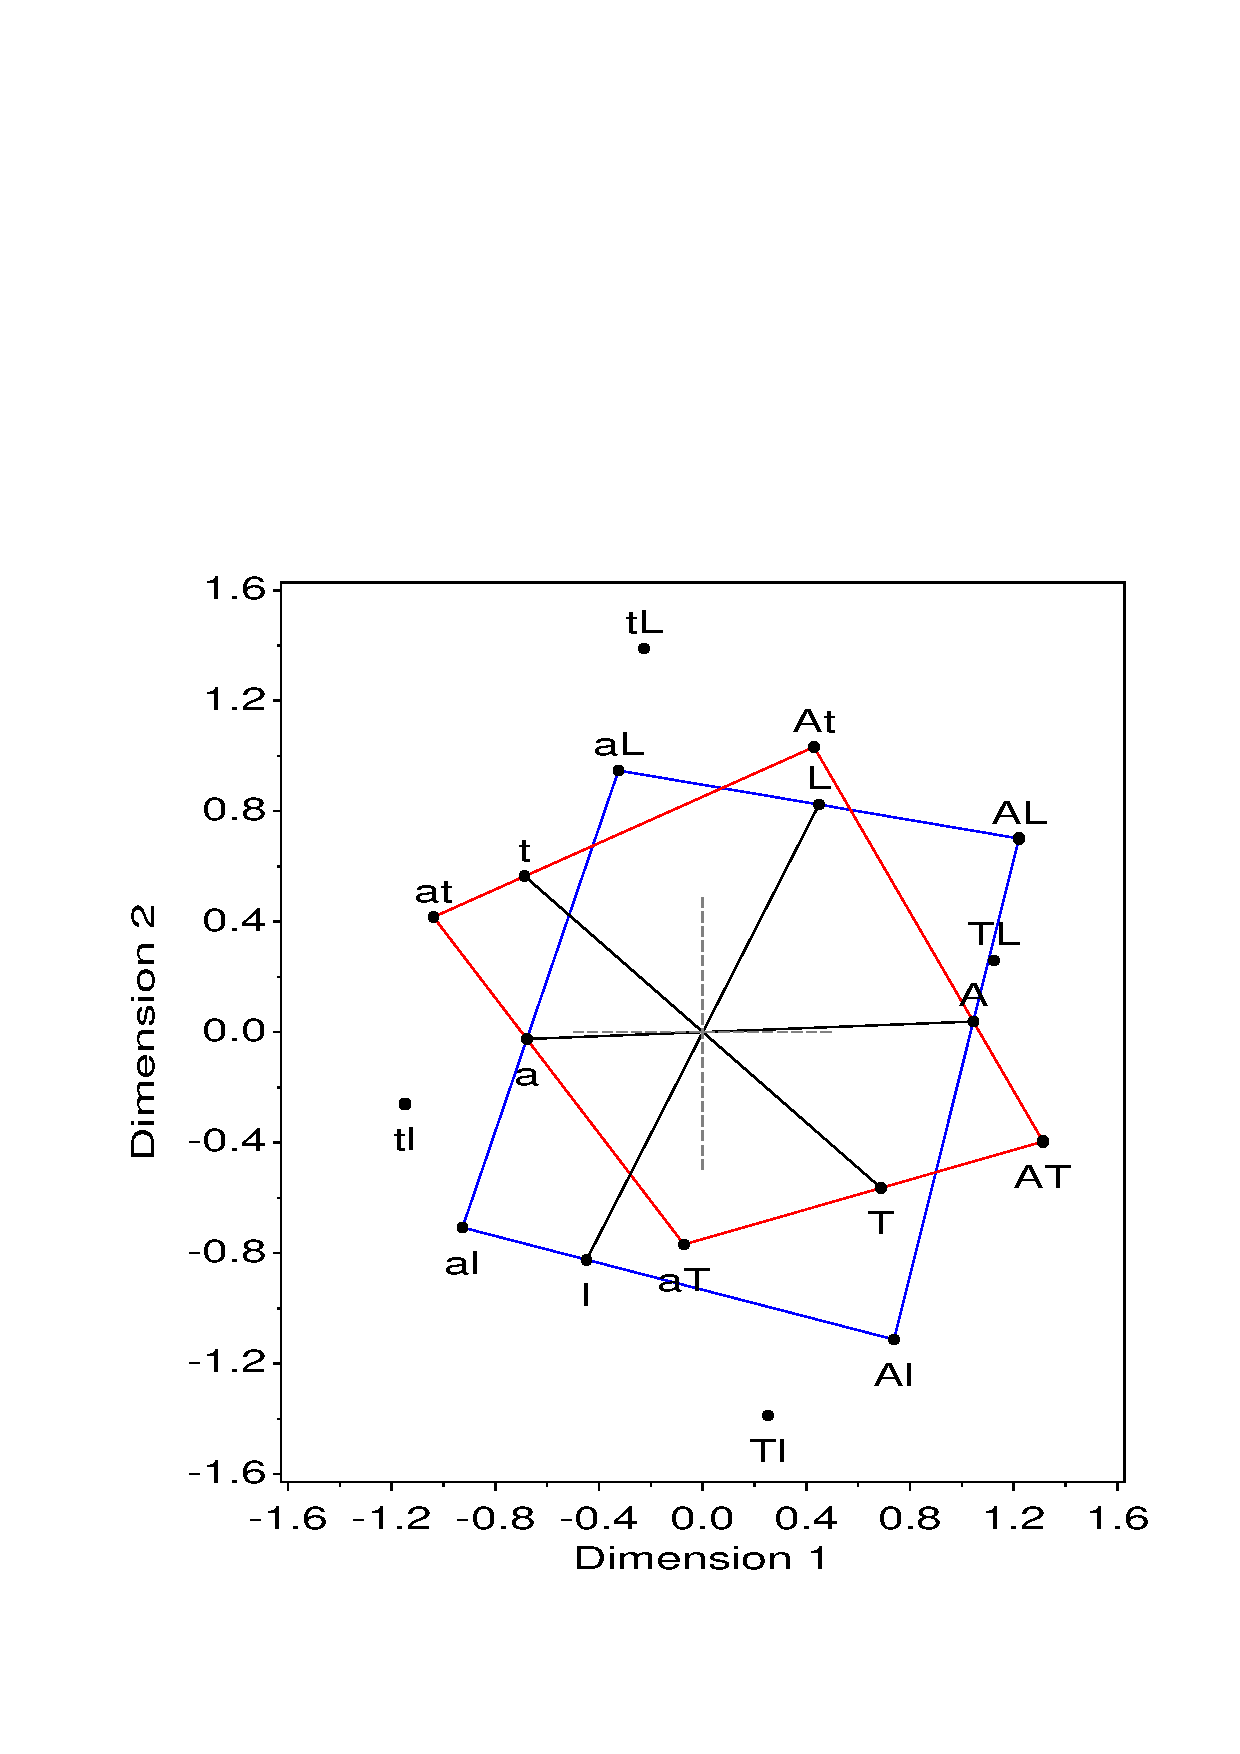
\includegraphics[width=1\linewidth]{ch5/fig/mcabart3}
 \end{minipage}
 \caption[2D Interaction display for Bartlett's data]{2D Interaction display for Bartlett's data.  Both panels show the same 2D solution for the MCA analysis including pairwise interaction effects.  In the left panel, points corresponding to the TL association are connected; lines joining the one-way
points are parallel to the sides, showing independence.
In the right panel, points for both the AT and AL associations are connected.}\label{fig:mcabart2}
\end{figure}
The following steps construct an \ADS\ to draw a quadrilateral for
each of the AT, AL and TL effects.
To do this, it is necessary to extract the \pname{DIM1} and \pname{DIM2}
of the four points for each effect and transpose these to a single
observation with variables \pname{X1-X4} and \pname{Y1-Y4} respectively.
The \Dset\ \pname{QUADS} created here is shown in \outref{out:mcabart4}
%% input: /users/faculty/friendly/sasuser/catdata/mcabart.sas
%% last modified: 16-Aug-98 12:31
\begin{listing}
*-- Extract x,y coordinates of two-way effects;
proc transpose data=coords(drop=_name_) out=quadx prefix=x;
   where (terms=2);
   var dim1;
   by effect;
proc transpose data=coords(drop=_name_) out=quady prefix=y;
   where (terms=2);
   var dim2;
   by effect;
data quads;
   merge quadx quady;
   drop _name_ _label_;
proc print data=quads;
   format _numeric_ 5.2;
   var x1 y1 x2 y2 x3 y3 x4 y4;
   id effect;

*-- Draw quadrilaterals, connecting points in order 1, 2, 4, 3;
data quads;
   set quads;
   drop x1-x4 y1-y4 i;
   retain xsys ysys '2';
   array xx\{*\} x1 x2 x4 x3;;
   array yy\{*\} y1 y2 y4 y3;
   color = scan('blue red green', _n_);
   do i=1 to 4;
      x = xx[i];  y=yy[i];
      if i=1 then function='poly    ';
             else function='polycont';
      output;
      end;

\end{listing}

\begin{Output}[htb]
\caption{\Dset\ \pname{QUADS}, containing the coordinates of the quadrilateral for each two-way effect}\label{out:mcabart4}
\begin{output}
   EFFECT     X1     Y1     X2     Y2     X3     Y3     X4     Y4

     AL     1.22   0.70   0.74  -1.11  -0.32   0.95  -0.93  -0.71
     AT     1.31  -0.40   0.43   1.03  -0.07  -0.77  -1.04   0.42
     TL     1.12   0.26   0.25  -1.39  -0.23   1.39  -1.15  -0.26
\end{output}
\end{Output}
The steps below complete the custom programming to display the TL
effect, with point labels and vectors for the main effects, in the left panel of \figref{fig:mcabart2}.
%% input: /users/faculty/friendly/sasuser/catdata/mcabart.sas
%% last modified: 16-Aug-98 12:31
\begin{listing}
%label(data=coords, out=label, x=dim1, y=dim2, text=_name_, pos=-);

data lines;
   set coords end=eof;;
   by terms effect notsorted;
   drop dim1 dim2 quality mass;
   x = dim1;
   y = dim2;
   xsys = '2'; ysys='2';

   if terms = 1  then do;
   color = 'black';
   if mod(_n_,2) = 1
      then do; function='MOVE    '; output; end;
      else do; function='DRAW    '; output; end;
   end;   

   if eof then do;
      color='gray'; line=3;
      x=-.5;  y=0;   function='MOVE';  output;   
      x=+.5;  y=0;   function='DRAW';  output;   
      x= 0 ;  y=-.5; function='MOVE';  output;   
      x= 0 ;  y=+.5; function='DRAW';  output;
      end;   
run;

*-- Show the Time X Length effect;
data anotes;
   set label lines quads(where=(effect in ('TL')));

proc gplot data=coords;
   plot dim2 * dim1 
      / frame vaxis=axis1 haxis=axis2 hm=1 vm=1
      anno=anotes;
   symbol1 v=dot h=1;
   axis1  length=6in order=(-1.6 to 1.6 by .4) label=(a=90);
   axis2  length=6in order=(-1.6 to 1.6 by .4);
run;
\end{listing}

The right panel of \figref{fig:mcabart2} is produced
using the same \PROC{GPLOT} step,
but the \ADS\ \pname{ANOTES} is assembled using just the
lines to connect the AT and AL points:
\begin{listing}
*-- Show effects on Alive;
data anotes;
   set label lines quads(where=(effect in ('AL' 'AT')));
proc gplot data=coords;
   ...
\end{listing}

Thus, we see that independence of Time and Length (by design of the
data collection) is characterized by a parallelogram shape for the
two-way points, and by lines joining the A and T one-way points
being parallel to those connecting the two-way points.
Note also that the one-way points are in essentially the same positions
as in \figref{fig:mcabart1}.
The quadrilaterals for the AT and AL effects shown in the right panel
are not quite parallelograms, however;  we could approximate the odds
ratio for each of these effects from the cross-product of distances
as in \eqref{eq:mcainter4}.
Finally, because one of the three quadrilaterals shows parallelism,
we conclude from \figref{fig:mcabart2} that the conditional independence
model, [AT][AL], holds.

An alternative representation allows us to show the cells instead, corresponding
to the ATL terms which were not displayed in \figref{fig:mcabart2}.
\begin{figure}[htb]
  \centering
  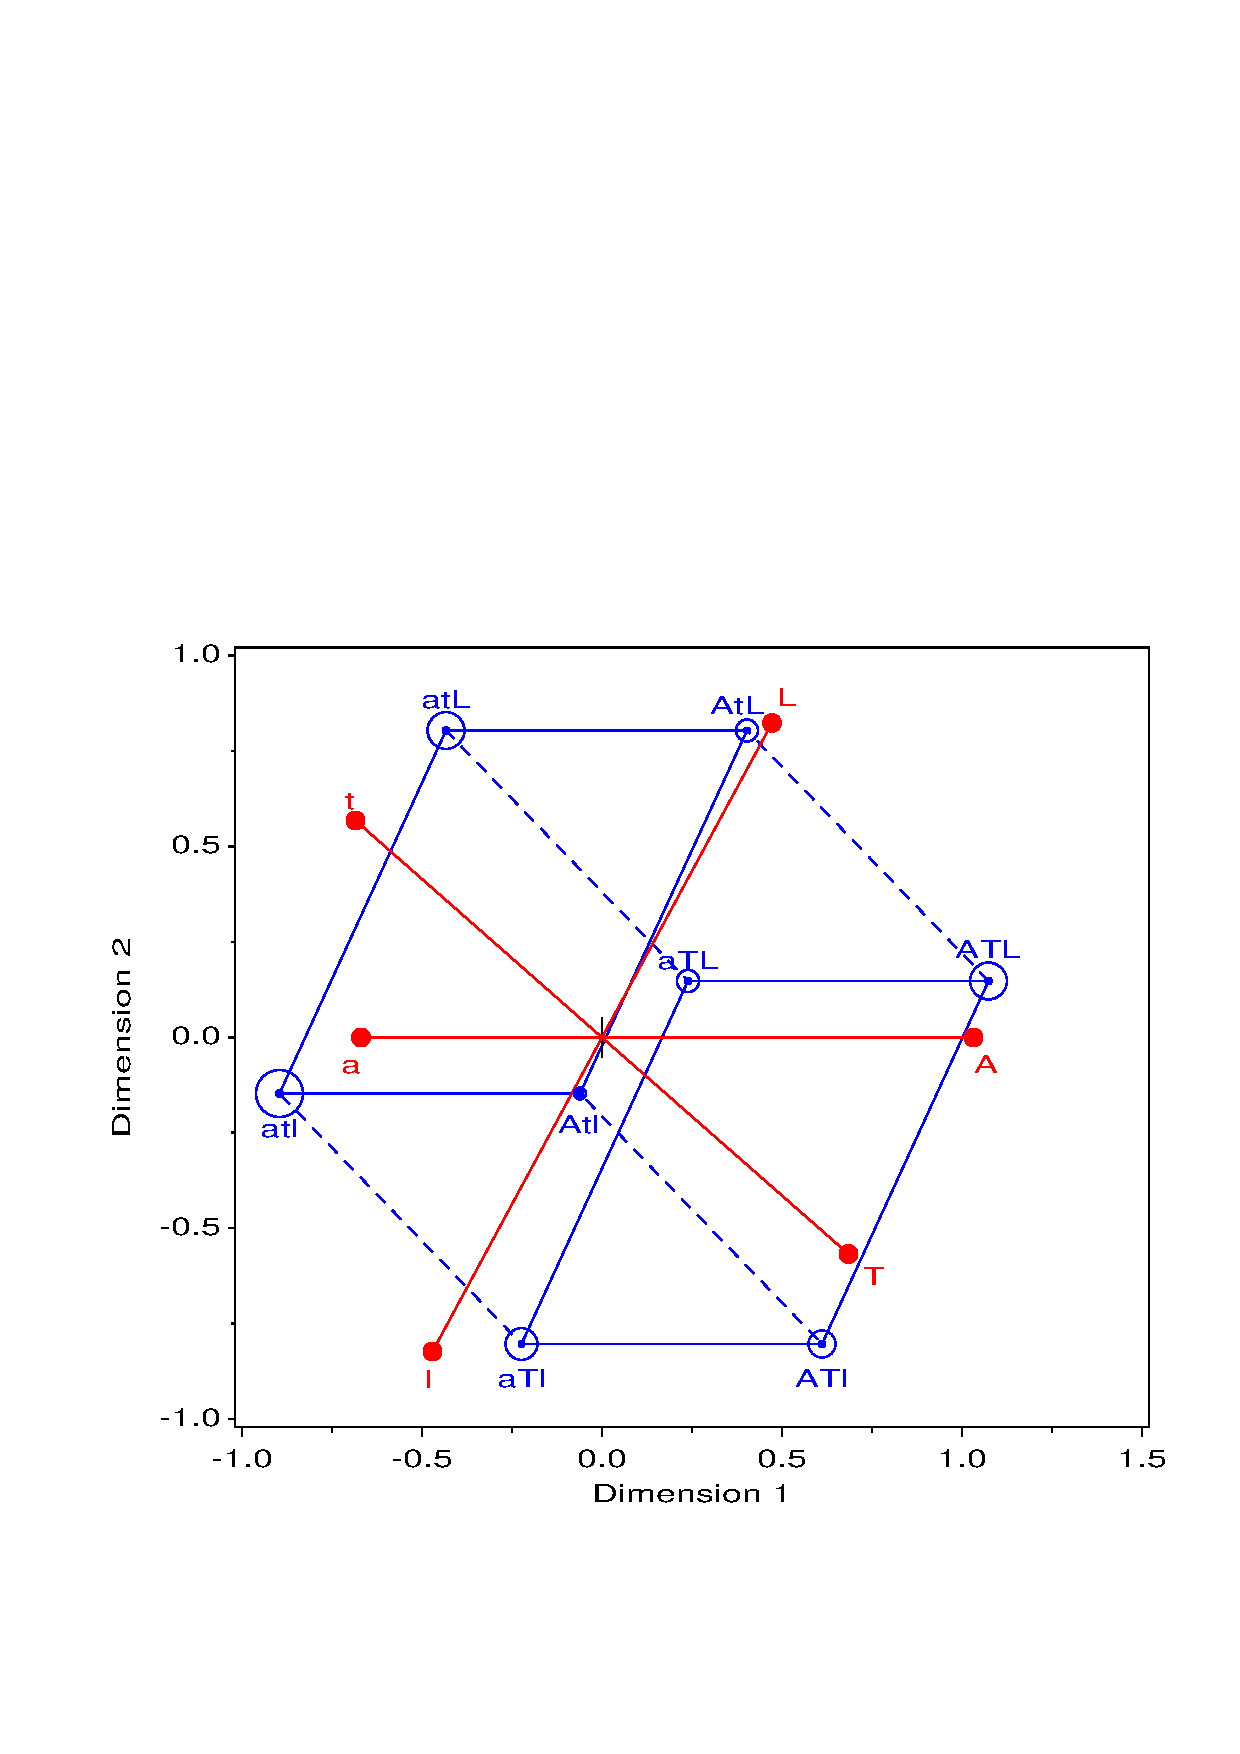
\includegraphics[scale=.7,clip]{ch5/fig/mcagen1}
  \caption[2D representation of the cell points in the $2\times 2 \times 2$ design]{2D representation of the cell points in the $2\times 2 \times 2$ design.  The mass (cell proportion) of each point is shown by the size of the circle.}\label{fig:mcagen1}
\end{figure}
We form the indicator matrix for the main effects,
$\mat{Z} = [
 \mat{Z}_A  \mat{Z}_T  \mat{Z}_L ]$,
and multiply by a diagonal matrix of the cell frequencies, to give:
\begin{output}
   ID    ALIVE   TIME     LENGTH   COUNT    A1    A2    T1    T2    L1    L2

   ATL   Alive   Now      Long      156    156     0   156     0   156     0
   aTL   Dead    Now      Long       84      0    84    84     0    84     0
   AtL   Alive   Spring   Long       84     84     0     0    84    84     0
   atL   Dead    Spring   Long      156      0   156     0   156   156     0
   ATl   Alive   Now      Short     107    107     0   107     0     0   107
   aTl   Dead    Now      Short     133      0   133   133     0     0   133
   Atl   Alive   Spring   Short      31     31     0     0    31     0    31
   atl   Dead    Spring   Short     209      0   209     0   209     0   209
\end{output}
Then, a simple \CA\ of the variables \pname{A1--L2} will have row points
corresponding to the cells, and column for the main effects which are
nearly identical to those from the extended MCA.
This analysis produces the display in \figref{fig:mcagen1}
(program steps are not shown to conserve space), where the
size of the circle at each point represents the mass ($p_{ijk}$) of each
cell, whose label is the \pname{ID} variable above.
The two-way points can be added to this representation by including the two-way indicator matrices, so we analyze the matrix
$\diag (\vec{n}) [
 \mat{Z}_A  \mat{Z}_T  \mat{Z}_L  \mat{Z}_{AT}
 \mat{Z}_{AL}  \mat{Z}_{TL}
]$.
\end{Example}
\ixoff{multiple correspondence analysis!extended}

